\documentclass{amsart}
\usepackage{amssymb,amsmath,amsthm,amsaddr}
\usepackage{thmtools}
\usepackage{thm-restate}

\usepackage{tikz,pgfplots,pgfplotstable}
\pgfplotsset{compat=1.9} % set to 1.8 to get old behaviour

%% %% % Graphics:
%% \usepackage[final]{graphicx}
\usepackage{graphicx} % use this line instead of the above to suppress graphics in draft copies
\usepackage{wrapfig}
%\usepackage{graphpap} % \defines the \graphpaper command
\usepackage[T1]{fontenc} % Use 8-bit encoding that has 256 glyphs
\usepackage[english]{babel} % English language/hyphenation


\usepackage{cite}
% makes color citations
\usepackage[colorlinks=true,urlcolor=blue,citecolor=red,linkcolor=red,bookmarks=true]{hyperref}
\usepackage{url}
\usepackage{color}
\usepackage{paralist}
%% \usepackage{graphics} %% add this and next lines if pictures should be in esp format
%% \usepackage{epsfig} %For pictures: screened artwork should be set up with an 85 or 100 line screen
\usepackage{epstopdf} 

%% From slides file
\usepackage{booktabs} % Allows the use of \toprule, \midrule and \bottomrule in tables
\usepackage[normalem]{ulem}
\usepackage{xcolor}
%\usepackage{algorithm}
%\usepackage[noend]{algpseudocode}
\usepackage{proof-at-the-end}

% Indent first line of each section:
\usepackage{indentfirst}

%% %% % Fonts and symbols:
\usepackage{amsfonts}


%% % Formatting tools:
%% %\usepackage{relsize} % relative font size selection, provides commands \textsmalle, \textlarger
%% %\usepackage{xspace} % gentle spacing in macros, such as \newcommand{\acims}{\textsc{acim}s\xspace}

%% % Page formatting utility:
%% \usepackage{geometry}
%% %\usepackage[margin=0.1in]{geometry}


%% Place here your \newcommand's and \renewcommand's. Some examples already included.
%\renewcommand{\le}{\leqslant}
%\renewcommand{\ge}{\geqslant}
%\renewcommand{\emptyset}{\ensuremath{\varnothing}}
%\newcommand{\ds}{\displaystyle}
\newcommand{\R}{\ensuremath{\mathbb{R}}}
%\newcommand{\Q}{\ensuremath{\mathbb{Q}}}
%\newcommand{\Z}{\ensuremath{\mathbb{Z}}}
%\newcommand{\N}{\ensuremath{\mathbb{N}}}
%\newcommand{\T}{\ensuremath{\mathbb{T}}}
%\newcommand{\B}{\mathcal{B}}
\newcommand{\eps}{\varepsilon}
%\newcommand{\closure}[1]{\ensuremath{\overline{#1}}}
\newcommand{\M}{\mathcal{M}}

\newcommand{\ep}{\varepsilon}
%\newcommand{\eps}[1]{{#1}_{\varepsilon}}
\newcommand{\bs}{\boldsymbol}
\newcommand{\der}{\text{\textup{d}}}
\newcommand{\coder}[1]{\texttt{#1}}
\newcommand{\inner}[2]{#1 \cdot #2}
\newcommand{\var}{\textup{Var}}
\newcommand{\corr}{\textup{Corr}}
\newcommand{\cov}{\textup{Cov}}
\newcommand{\diag}{\textup{diag}}
%% \newcommand{\dom}{\mathcal{D}om}
%% \newcommand{\note}[1]{{\textcolor{blue}{#1}}}
%% \newcommand{\A}[1]{{\textcolor{cyan}{\noindent Answer: #1}}}
%\newcommand{\reftwo}[1]{{\textcolor{green}{#1}}}
%\newcommand{\refthree}[1]{{\textcolor{red}{#1}}}
%% \newcommand{\refthree}[1]{{\color{red} #1}}
%% \newcommand{\reftwo}[1]{{\color{green} #1}}



%% \newcommand{\precop}{\mathcal{L}}
%% \newcommand{\precmat}{\mathbf{L}}
%% \newcommand{\Op}{\mathcal{A}}
%% \newcommand{\OpDir}{\mathcal{A}_{\textup{Dirichlet}}}
%% \newcommand{\OpNeu}{\mathcal{A}_{\textup{Neumann}}}
%% \newcommand{\covop}{\mathcal{C}}
%% \newcommand{\lag}{\mathcal{L}}
%% \newcommand{\n}{\boldsymbol{n} }
%% \newcommand{\dn}{\partial \n }
\newcommand{\x}{\mathbf{x}}
\newcommand{\y}{\mathbf{y}}
%% \newcommand{\z}{{\boldsymbol{z}}}
%% \newcommand{\kxmy}{ \kappa \| \x - \y \| }
%% \newcommand{\xmy}{ \| \x - \y \| }
%% \newcommand{\proj}{\mathcal{P}}
%% \newcommand{\kr}{\kappa r}
%% \newcommand{\ivar}{\text{IntVar}}

%% \newcommand{\K}{\mathbb{K}}
\newcommand{\hil}{\mathcal{H}}
%% \newcommand{\ban}{\mathcal{B}}
\newcommand{\hilp}{\mathcal{H}_p}
\newcommand{\hilo}{\mathcal{H}_o}
\newcommand{\obs}{\mathcal{O}}
\newcommand{\pobs}{\mathcal{P}}
\newcommand{\fwd}{\mathcal{F}}
%% \newcommand{\tru}{\fwd_{\textup{True}}}
%% \newcommand{\err}{\fwd_{\textup{Error}}}

\newcommand{\obsm}{\widehat{\obs}}
\newcommand{\Sigmam}{\widehat{\Sigma}}
\newcommand{\postcovm}{\widehat{\Gamma_{\textup{post}}}}
\newcommand{\uu}{\mathbf{u}}
\newcommand{\tar}{\Psi}
\DeclareMathOperator*{\argmin}{arg\,min}
\DeclareMathOperator*{\argmax}{arg\,max}

% Definitions for second chapter
\newcommand{\data}{\mathbf{d}}
\newcommand{\param}{\mathbf{m}}
\newcommand{\sspar}{\param_{\textup{SmallScale}}}
\newcommand{\normal}{\mathcal{N}}
\newcommand{\pr}{\mu_{\textup{pr}}} %Prior measure
\newcommand{\post}{\mu_{\textup{post}}^{\data, \obs}} % Posterior measure
\newcommand{\prmean}{\param_{\textup{pr}}} % Prior mean
\newcommand{\postmean}{\param_{\textup{post}}} % Posterior mean
\newcommand{\postcov}{\Gamma_{\textup{post}}} % Posterior covariance
\newcommand{\prcov}{\Gamma_{\textup{pr}}} % Prior covariance
\newcommand{\modcov}{\Gamma_{\textup{model}}} % Model covariance
\newcommand{\tmp}{\mathcal{G}}
\newcommand{\meas}{\mathbf{o}}
\newcommand{\ev}{\mathbf{e}} % eigenvector 
\newcommand{\func}{\mathbf{a}}
\newcommand{\tr}[1]{\textup{tr}\left \{#1 \right \} }
\newcommand{\ttr}[1]{\textup{tr}\ #1}
\newcommand{\rank}{\textup{rank}\ }
\newcommand{\des}{\eta} % vector of design parameters
\newcommand{\sigsqr}{\sigma^2}
%\newcommand{\acim}{\textsc{acim}\xspace}
%\newcommand{\acims}{\textsc{acim}s\xspace}


%% %% \newcommand\numberthis{\addtocounter{equation}{1}\tag{\theequation}}
%% %% %%
%% %% %% Place here your \newtheorem's:
%% %% %%
\newtheorem{theorem}{Theorem}
\newtheorem{definition}{Definition}

%% %% %% Some examples commented out below. Create your own or use these...
%% %% %%%%%%%%%\swapnumbers % this makes the numbers appear before the statement name.
%% %% %\theoremstyle{plain}
%% %% %\newtheorem{thm}{Theorem}[chapter]
\newtheorem{proposition}{Proposition}
\newtheorem{lemma}{Lemma}
\newtheorem{corollary}{Corollary}
%% %% % \newtheorem{observation}[theorem]{Observation}

%% %% %\theoremstyle{definition}
%% %% %\newtheorem{define}{Definition}[chapter]

%% %% %\theoremstyle{remark}
%% %% %\newtheorem*{rmk*}{Remark}
%% %% %\newtheorem*{rmks*}{Remarks}

%% %% %% Hack
%% %% \newcommand{\stkout}[1]{\ifmmode\text{\sout{\ensuremath{#1}}}\else\sout{#1}\fi}
%% %% \usepackage{cancel}

\usepackage{comment}% http://ctan.org/pkg/comment
%% %% %\excludecomment{proof}
%% \excludecomment{figure}
%% \let\endfigure\relax


\overfullrule=0pt


\numberwithin{equation}{section}

\begin{document}

\title[Sensor Clusterization in D-optimal design in infinite
  dimensions]{Sensor Clusterization in D-optimal Design in Infinite
  Dimensional Bayesian Linear Inverse Problems}

\author{Yair Daon}
\address{Porter School of the Environment and Earth
  Sciences, Tel Aviv University\\ Tel Aviv, Israel}
%% \curraddr{Porter School of Environment Studies, Tel Aviv University\\ Tel Aviv, Israel}
%% \curraddr{}
\email{yair.daon@gmail.com}
%% \thanks{}

%    The 2010 edition of the Mathematics Subject Classification is
%    the current definitive version.
\subjclass{Primary: 
  62F15, % Statistics - bayesian inference
  35R30, % PDE - Inverse problems
  Secondary:
  28C20, % Measure and integration - set functions and measures and integrals in
  %infinite-dimensional spaces (Wiener measure, Gaussian measure, etc.
}
%% Primary: 62F15, 35R30; Secondary: 28C20
\date{\today}

\begin{abstract}
  We investigate the problem of sensor clusterization in D-optimal
  experimental design for infinite-dimensional Bayesian linear inverse
  problems. We suggest an analytically tractable model for D-optimal
  designs and reason how it may lead to sensor clusterization in the
  case of iid observation noise. We also consider how spatially
  correlated observation and model errors mitigate the clusterization
  phenomenon.

  %% As a part of the analysis we prove a Matrix Determinant
  %% Lemma in Hilbert spaces and a lemma for calculating
  %% $\frac{\der}{\der t} \log \det (I + X(t))$ for certain
  %% operator-valued functions. We also show how to decompose $M = AA^t$
  %% with $A$ constrained to have unit norm columns.
\end{abstract}

\maketitle

\section{Introduction}\label{section:OED intro}
Experimental design is an important part of many scientific
investigations. When considering an inverse problem, one can often
specify sensor locations (e.g.\ in geophysics and oceanography
applications), certain wavelengths (e.g.\ in MRI) or wave reflections
from the ground (e.g.\ searching for oil or using a radar). Whatever
the allowed set of observations is, one should select the optimal
observations to take, in order to increase accuracy, reduce costs, or
both.

Designing experiments is usually done by optimizing some \emph{design
  criterion}. This is true both for frequentists
\cite{Silvey13,Ucinski05} as well as for Bayesians
\cite{ChalonerVerdinelli95}. See \cite{ChalonerVerdinelli95} for an
investigation of the analogy between the two approaches. Although
there is a plethora of design criteria, we focus on just one of these,
commonly referred to as \emph{D-optimal design}. It has a simple and
appealing motivation in the Bayesian context as explained in
\cite{ChalonerVerdinelli95}: Consider a linear model in finite
dimensions, with Gaussian prior and noise. Under this model,
maximizing the expected information gain (KL divergence
\cite{KullbackLeibler51,CoverThomas12}) between posterior and prior
amounts to minimizing the determinant of the posterior covariance
matrix. In a frequentist setting, a D-optimal design minimizes the
volume of the uncertainty ellipsoid \cite[page 16]{Ucinski05}, but
this is done for the Fisher information matrix and not the posterior
covariance. However, \cite{ChalonerVerdinelli95} shows that the latter
is just a regularized version of the former.

The previous discussion is classical for experimental design when
inference takes place over a finite (not too large) number of
parameters. The subject of optimal experimental design for function
inference in a Bayesian context was pioneered by
\cite{AlexanderianGloorGhattas14, AlexanderianPetraStadlerEtAl16,
  AlexanderianPetraStadlerEtAl14}. Similarly to the finite dimensional
case, it can be shown that a D-optimal design arises naturally for
linear models when one wishes to maximize the KL divergence between
posterior and prior. This amounts to minimizing the determinant of the
posterior covariance operator (understood as a product of its
eigenvalues). Some difficulties arise in the process, but remedies can
be found as shown in \cite{AlexanderianGloorGhattas14}.

It seems counter intuitive that when one computes an optimal design
using the D criterion, the optimization process results in
observations that are very similar. For example, if an observation is
thought of as measuring some function value at $\x \in \Omega
\subseteq \R^d, d=1,2,3$ (with added error) then the optimization
procedure sometimes places sensors in very close proximity to each
other (as can be seen in figure \ref{fig:clusterization
  illustration}). Following \cite{Ucinski05}, we refer to this
phenomenon as \emph{sensor clusterization}.

\subsection{Related Work}
The phenomenon of sensor clusterization seems to be known in several
different contexts. In a frequentist and finite-dimensional context,
\cite{Fedorov96} and \cite[chapter 2.4.3]{Ucinski05} discuss this
phenomenon and suggest an approach called clusterization-free design.
In such designs, the user enforces observation locations to be far
from each other. One way to do this is by introducing correlated
errors which, philosophically, accounts for both observation error and
model error. Another method considered is imposing distance
constraints between observations. A somewhat different approach is
suggested in \cite[page 49]{Fedorov12}, where close by design
observations are merged --- a procedure which obviously does not avoid
clusterization. The same problem arises in time-series analysis for
pharmacokinetic experiments. The authors of \cite{Hooker09} suggest
modeling auto-correlation time in the noise model, which is equivalent
to the correlated errors mentioned above.

Any of the above mentioned approaches might serve as a remedy and push
sensors away from each other. Yet, none offers any insight as to why
clusterization occurs. Also, as better models are employed, model
error is decreased and the clusterization phenomenon will eventually
reappear. While these approaches are practical and help us avoid the
problem, they do not provide insight as to why sensors are clustering.

Similarly, in the inverse problems community, work is mostly
computational and less theoretic. Model errors were considered in
\cite{Attia20, Koval20}. The former study is focused on inferring a
Quantity of Interest (QoI). The focus of the latter is reducing
forward solves, using randomized linear algebra. Both studies present
numerical techniques for finding optimal designs when model error is
present. Both are restricted to linear inverse problems (although in
the latter the authors use their method on a nonlinear problem by
taking a Laplace approximation for the posterior). Both find an
optimal design by first solving a continuous problem for sensor
weights. Said solution is then sparsified to give a binary
design. Both studies are successful in the task of Bayesian
inversion. However, neither of these studies mention any effect model
errors can have on sensor clusterization. The current study is mostly
theoretical and aims to fill the gap of understanding sensor
clusterization.


\subsection{Contribution}
We propose and thoroughly study a relaxed and analytically tractable
model for understanding D-optimal designs. Under this model, D-optimal
designs are solutions of a constrained optimization problem,
formulated using Lagrange multipliers (section \ref{section:D and
  grad}). This allows us to rigorously show how model error mitigates
clusterization (section \ref{section:non vanishing}). We show how
clusterization occurs in a sequential design scenario (section
\ref{subsec:clusterization sequential}). Then, we consider a
simultaneous D-optimal design scenario (section
\ref{subsec:clusterization simultaneous}). We show that designs that
exhibit clusterization are just as optimal as clusterization free
designs.

A beautiful mathematical structure arises in D-optimal designs when no
model error is present. The Lagrange multipliers problems is in fact a
nonlinear eigenvalue problem for the observations and prior
covariance. The operator for which eigenvectors and eigenvalues are
sought is a sum of two operators. The first is the prior
covariance. The second is an outer product of the observations (see
section \ref{section:vanishing} for details and exact statement). This
structure helps us shed light on D-optimal designs. We characterize
these designs in Theorem \ref{thm:char}. One insight we prove is that
a D-optimal design reduces uncertainties where they are highest
first. Other interestig phenomena arise, but they require setting
notation, and are discussed later.

In the process, we generalize several lemmas from linear algebra to
infinite-dimensional settings. We prove a Matrix Determinant Lemma in
\ref{lemma:MDL}. We generalize a lemma due to Lax \cite{lax97} for
calculating $\frac{\der}{\der t} \log \det (I + X(t))$, for an
operator valued function $X(t)$ in \ref{lemma:lax}. We also prove
lemmas in linear algebra. One constructs a decomposition $M = AA^t$
where $A$ has unit norm columns \ref{lemma:free}. Another shows
simultaneous diagonizability of the prior and outer product in the
nonlinear eigenvalue problem referenced above \ref{lemma:sim diag}. We
also provide other tools for understanding D-optimal designs in
infinite-dimensional Bayesian inverse problems. These include tools
for calculating the increase in the design criterion per observation
--- Lemma \ref{lemma:design increase} and Corollary \ref{cor:zero mod
  err}.

\begin{restatable}[D-optimal designs with vanishing model error]{theorem}{main}\label{thm:char}
  Let:
  \begin{enumerate}
  \item $\fwd:\hilp \to \hilo$ a linear forward operator,
    $\prcov:\hilp \to \hilp$ prior covariance operator, $\obs: \hilo
    \to \mathbb{R}^m$ observation operator, where $m \in \mathbb{N}$
    is the number of observations taken.
    \item $\sigma^2 \in \mathbb{R}_{+}$ observation noise variance,
      $\data = \obs \fwd \param + \eps$, where $\eps \in \mathbb{R}^m$
      is iid $\mathcal{N}(0, \sigma^2)$ noise, $\pr \sim
      \mathcal{N}(0, \prcov)$ prior measure, $\post$ the posterior
      measure.
  \item A D-optimality utility function
    \cite{AlexanderianGloorGhattas14}:
    \begin{align*}
      \begin{split}
        \tar(\obs) :&= \mathbb{E}_{\data}\left [ D_{\text{KL}} (\post || \pr ) \right ] \\
        % 
        % 
        % 
        &= \frac12 \log \det ( I + \sigma^{-2} \prcov^{1/2} \fwd ^*
        \obs^* \obs \fwd \prcov^{1/2}).
    \end{split}
  \end{align*}
  \item A D-optimal design operator $\obs$:
    $$
    \obs = \argmax_{\|\meas_j\| = 1, j=1,\dots,m}\tar(\obs)
    $$ 
  \item $\{\lambda_i\}_{i=1}^\infty$ eigenvalues of $\fwd\prcov\fwd^*$
    in decreasing order of magnitude.
  %% \item $\{\ev_i\}_{i=1}^\infty$ their corresponding eigenvectors.
  \item $\{\eta_i\}_{i=1}^\infty$ eigenvalues of $\obs^*\obs$.
  \end{enumerate}

  Then:
  \begin{enumerate}
  \item $\obs^*\obs$ and $\fwd\prcov\fwd^*$ are simultaneously
    diagonalizable.
  \item $k := \rank \obs^*\obs \leq m$.
  \item     
    \begin{equation*}
      \tar(\obs) = \frac12 \sum_{i=1}^{k} \log (1 + \sigma^{-2}\lambda_i\eta_i). %= \frac12 \sum_{i=1}^{m} \log (1 + \sigma^{-2}\lambda_i\eta_i).
    \end{equation*}
  %% \item 
  %%   \begin{equation*}
  %%     k = \argmax \left \{ k:\lambda_k^{-1} < \sigma^{-2}\frac{m}{k} + \frac{1}{k} \sum_{j=1}^{k}
  %%     \lambda_j^{-1} \right \}.
  %%   \end{equation*}
  \item
    \begin{equation*}
        \eta_i = \begin{cases}
          \frac{m}{k} - \sigma^2 \lambda_i^{-1} + \sigma^2 \frac{1}{k} \sum_{j=1}^k \lambda_j^{-1} & 1 \leq i \leq k \\
          0 & i > k 
        \end{cases}.
    \end{equation*}
  \end{enumerate}
\end{restatable}

\subsection{Limitations}\label{subsec:limitations}
There are two main drawbacks of the study presented here. Our relaxed
model does not consider any specific set of allowed
observations. Rather, we take observations in the unit ball in some
Hilbert space. This allows considerably less restrictive observations
than any real-life problem does. The second drawback is that we do not
show rigorously that clusterization necessarily occurs in a
simultaneous design. We only show that it is as reasonable as no
clusterization.


\subsection{An Example of Clusterization}\label{subsec:example}
\begin{figure}
  \begin{tikzpicture}[thick, scale=1.3, every node/.style={scale=0.99}]
    \begin{axis}
      [
      title={Posterior Pointwise Standard Deviations and D-Optimal Sensor Locations},  
      xmin = 0,
      xmax = 3.14,
      xlabel = {$x$},
      ylabel = posterior std,
      ymin   = 0,
      %compat = 1.3,
      % ymax   = 130,
      % ytick = \empty,
      legend cell align=left,
      % legend style={at={(0.45,0.2)}}
      legend pos= outer north east 
      ]
      % \draw[black!30!white, thin] (50,0) -- (50,130);
      % 
      %% \addplot [thin, black, mark=none] table{stdv-heat-sens1-var1.txt};
      %% \addlegendentry{1 sensors};
      
      %% \addplot [thin, blue, mark=none] table{stdv-heat-sens2-var1.txt};
      %% \addlegendentry{2 sensors};
      
      %% \addplot [thin, red, mark=none] table{stdv-heat-sens3-var1.txt};
      %% \addlegendentry{3 sensors};
      
      \addplot [thin, green, mark=none] table{stdv-heat-sens4-var1.txt};
      \addlegendentry{4 sensors};
      
      \addplot [thin, purple, mark=none] table{stdv-heat-sens5-var1.txt};
      \addlegendentry{5 sensors};
      
      \addplot [thin, cyan, mark=none] table{stdv-heat-sens6-var1.txt};
      \addlegendentry{6 sensors};

  
      %% \addplot [black,  only marks, mark=x, mark size=1.5] 
      %% table{locs-heat-sens1-var1.txt}; 
      %% \addplot [blue,   only marks, mark=x, mark size=1.5]
      %% table{locs-heat-sens2-var1.txt}; 
      %% \addplot [red,    only marks, mark=x, mark size=1.5]
      %% table{locs-heat-sens3-var1.txt};
      \addplot [green,  only marks, mark=*, mark size=1.5] 
      table{locs-heat-sens4-var1.txt}; 
      \addplot [purple, only marks, mark=*, mark size=1.5] 
      table{locs-heat-sens5-var1.txt}; 
      \addplot [cyan,   only marks, mark=*, mark size=1.5] 
      table{locs-heat-sens6-var1.txt}; 
  
      
    \end{axis}
  \end{tikzpicture}
  \caption{The clusterization effect for the 1D heat equation
    described in section \ref{subsec:example}. Posterior pointwise
    standard deviations (lines) are plotted over the domain $[0,
      \pi]$, for varying numbers of sensors. Sensor locations
    (circles) were chosen to minimize (an expression analogous to) the
    determinant of the posterior covariance. The clusterization effect
    can be clearly seen for six sensors. Only four observation
    locations are used --- two pairs of sensors are so close they are
    indistinguishable.}
  \label{fig:clusterization illustration}
\end{figure}

In section \ref{section:prelim} we present a more abstract and general
formulation of the inverse problem we consider. But, for the purpose
of illustration, we present clusterization via a toy model --- the 1D
heat equation in $[0,\pi]$ with a homogeneous Dirichlet boundary
condition.

The 1D heat equation is:
\begin{subequations}\label{eq:heat equation}
  \begin{alignat}{2}
    u_t &= \Delta u &&\qquad \text{in } [0,\pi] \times [0,\infty),\\
      u &= 0 &&\qquad \text{on } \{0, \pi\} \times [0,\infty),\\
        u &= u_0 &&\qquad \text{on }[0,\pi] \times \{0\}.
  \end{alignat}
\end{subequations}

We would like to infer the initial condition $u_0$. For that purpose,
we measure $u$ at some set of locations $\x_j \in [0,\pi], j=1,
\dots,m$ and a final time $T > 0$. We assume centered Gaussian
observation error, so we observe $v(\x_j,T) = u(\x_j,T) + \eps(\x_j)$
with $\eps(\x_j) \sim \normal(0, \sigma^2), \sigma > 0$ iid. We model
the initial condition as $u_0 \sim \normal(0,\prcov)$, for $\prcov =
(-\Delta)^{-1}$ with a homogeneous Dirichlet boundary condition. If It
is well known \cite{Tarantola05} that for linear problems, with
Gaussian prior and error, the posterior is also Gaussian with a
covariance that does not depend on the observed data. The posterior
covariance $\postcov$ is known to have a closed form formula, even in
infinite dimensions\cite{Stuart10}. We denote by $\fwd$ the dynamics
operator, so that $u( \cdot,T) = \fwd u_0$, and the observation
operator $\obs$ so that $u(\x_j,T) = (\obs u)_j, j=1,\dots,m$. The
posterior covariance is known and depends only on $\prcov, \fwd, \obs$
and $\sigma^2$ (see section \ref{section:prelim} and
\eqref{eq:postcov} specifically).

We consider generalization of the information-theoretic design
criterion presented in the introduction to infinite dimensions
(section \ref{subsec:D optimal design} below). We choose
$\x_j,j=1,\dots,m$ to minimize (an expression analogous to) the
determinant of the posterior covariance operator. We will see later
how this corresponds to maximizing expected information gain.

The clusterization effect is illustrated in figure
\ref{fig:clusterization illustration}. Posterior pointwise standard
deviations are plotted over the domain $[0, \pi]$. Since the posterior
covariance does not depend on data, the plot has no reference to
actual data observed. The posterior covariance does, however, depend
on location of the observation taken. In figure
\ref{fig:clusterization illustration}, observation locations are
marked by circles. These were chosen to minimize (an expression
analogous to) the determinant of the posterior covariance. The
clusterization effect can be clearly seen for six sensors. It looks
like only four observations were taken. The reason is that two pairs
of sensors are so close they are indistinguishable.


\section{Preliminaries and Notation}\label{section:prelim}

\subsection{Overview}
In this section we define notations that will be used throughout the
paper. The theoretical foundations for inverse problems over function spaces
can be found in \cite{Stuart10}.


\subsection{Bayesian Linear Inverse Problems}\label{subsec:abstract OED}
Let $\hilp$ and $\hilo$ be separable Hilbert spaces (the subscripts p
and o are for ``parameter'' and ``observation'', respectfully). We
denote $\hilo^*$ the Hilbert space of all linear functionals on
$\hilo$. Consider $\fwd: \hilp \to \hilo$, a linear operator (the
``forward operator''). We are interested in forward operators that are
strongly smoothing (have fast decaying modes --- the heat operator
from section \ref{subsec:example} is a prime example). Our goal is to
infer $\param \in \hilp$ --- some parameter of the dynamics --- given
noisy observations of $\fwd \param$. We take a Gaussian prior $\pr$
for $\param$. Hence, $\param \sim \pr = \normal(\prmean ,\prcov)$ with
some appropriate covariance operator $\prcov$ \cite{Stuart10}. It is
important to note that $\fwd \prcov \fwd^*$ is the prior covariance in
$\hilo$ \cite{Stuart10}. As such, it is assumed invertible --- an
assumption we rely on below. Throughout this paper, we denote $m$ the
number of observations we are allowed to take. Observations are taken
via the operator $\obs \in ( \hilo^* )^m$. In an analogy with linear
algebra, where row vectors are thought of as linear functionals, we
think of $\obs$ as having ``rows'' $\meas_j, j=1,\dots,m$:
\begin{equation}\label{eq:O}
  \obs = (\meas_1,\dots, \meas_m)^t, \meas_j \in \hilo^*, j = 1,\dots,m.
\end{equation}
This way, for $u \in \hilo$ we have $\obs u = (\meas_1(u), \dots,
\meas_m(u) )^t \in \R^m$.
%% but we may drop the parentheses and write $\meas_j u = \meas_j(u)$.
%% A few observations regarding $\obs$ are in order.
%% First, it is good to keep in mind that $( \hilo^* )^m$ is a Hilbert
%% space with norm $\| \obs \| = \sum_{j=1}^m \|\meas_j\|$.
For $u \in \hilo$ and $v\in \R^m$:
\begin{align*}
  \big (\obs^*v \big ) (u) &= \langle v, \obs u \rangle_{\R^m} = \sum_{j=1}^m  v_j \meas_j(u)
  = v^t \left ( \obs u \right ) = (v^t \obs) (u),
\end{align*}
and thus:
\begin{align}\label{eq:obs*}
  \obs^*v &= \sum_{j=1}^m v_j \meas_j = v^t \obs.
\end{align}

%% \begin{observation}
%%   It is best to think of $\meas_j,j=1,\dots,m$ as row vectors and of
%%   $\obs$ as a matrix with rows $\meas_j$. 
%% \end{observation}

Each observation is a linear functional, chosen from some subset of
$\hilo^{*}$. Data is acquired via noisy observations
\begin{align}\label{eq:inverse problem}
  \data := \obs (\fwd \param + \eps') + \eps = \obs \fwd \param + \obs \eps' + \eps,
\end{align}
with $\data \in \R^m$ and $\eps, \eps'$ defined next. We consider two
types of error terms. First, there is spatially correlated model error
$\eps' \sim \normal(0,\modcov)$, modeled as a centered Gaussian
measure on $\hilo$ with covariance operator $\modcov$. Then there is
observation error $\eps \sim \normal(0, \sigma^2 I_m)$, with $I_m$ the
$m \times m$ identity. Both error terms and the prior are assumed
independent of each other. The observation and forward operators are
typically merged $\tmp := \obs \fwd$
\cite{AlexanderianGloorGhattas14}. Since we need to separate the
observation operator $\obs$ from the forward operator $\fwd$ in order
to carry out the analysis in the following sections, we explicitly
separate $\fwd$ and $\obs$ in \eqref{eq:inverse problem}. We now turn
to understand the terms present in \eqref{eq:inverse problem}.


\subsubsection{Dynamics and Observation Operators}\label{subsec:dynamics}
Rows of $\obs$ are linear functionals and we refer to these as {\it
  observation vector}s. Note that we cannot choose every observation
vector we want. For example, we may be restricted only to pointwise
evaluations of $\fwd \param$ by the sensors at our disposal, in which
case measuring, e.g., the mean $\ell(u) = \int_{\Omega}u$ of a
function is not possible. Thus, it is best to think of $(\obs \fwd
\param)_j$ as approximations to pointwise evaluations. For example, if
$\hilo = L^2([-\pi, \pi])$, consider $\ell_1(x) := (2\pi
\eps)^{-\frac{1}{2}}\exp(-\frac{x^2}{2\eps^2})$ and $\ell_2(x)
:=\eps^{-1}\mathbf{1}_{[-\frac{\eps}{2}, \frac{\eps}{2}]}$. Both
$\ell_1$ and $\ell_2$ approximate a point measurement at $0$ for small
$\eps$ and, crucially, $\ell_1, \ell_2 \in \hilo^*$. It is important
to note that although $\|\ell\|_1 = \|\ell_2\|_1=1$, unfortunately
$\|\ell_1\|_2^2 = (4\pi \eps)^{-\frac{1}{2}}$ and $\|\ell_2\|_2^2 =
\eps^{-1}$.


\subsubsection{Error Terms}
Considering the sum of the error terms, it is easy to see that
$\bar{\eps} := \obs \eps' + \eps \in \R^m$. It is a centered Gaussian
random vector and its covariance matrix is
\begin{align}\label{eq:Sigma}
  \begin{split}
    \Sigma(\obs) :&= \mathbb{E}[ (\obs \eps' + \eps)  (\obs \eps' + \eps)^t ] 
    % 
    % 
    = \obs \modcov \obs^* + \sigma^2I , 
  \end{split}
\end{align}
where
\begin{equation}\label{eq:modcov explained}
  [\obs \modcov \obs^*]_{ij} = e_i^t \obs \modcov \obs^* e_j = \meas_i (\modcov \meas_j),
\end{equation}
with $e_j \in \R^m$ the $j$th standard basis vector. The first
equality in \eqref{eq:modcov explained} holds by definition and the
second by \eqref{eq:obs*}. The explicit dependence on $\obs$ will be
mostly dropped for notational convenience, so $\Sigma(\obs) =
\Sigma$. Thus, for a fixed $\obs$ (i.e.\ a fixed set of observations)
we can equivalently write $\data = \obs \fwd \param + \bar{\eps}$ with
$\bar{\eps} \sim \normal(0,\Sigma)$. Taking $\modcov = 0$ is common
practice \cite{Tarantola05,KaipioSomersalo05,Vogel02}. This reduces to
the case where we take iid observations. Then $\Sigma = \sigma^2I$ is
simply a scalar matrix that does not depend on $\obs$. Note that
taking an error model with a non-scalar covariance as we do here
allows us to consider model error (modeled by $\modcov$) as well as
observation error (modeled by $\sigma^2$). For example, say we believe
our forward model does not capture some small scale phenomenon.  Then
we may express this belief by saying $\tru = \fwd + \err$, with $\fwd$
depending on $\param$ and $\err$ depending on $\sspar$, with $\param
\perp \sspar$. We do not know much about this effect but it is
reasonable to assume it changes continuously in our domain. We (may
choose to) model it as $\normal (0, \modcov)$ and take $\modcov$ to
reflect the spatial (or other) variability we imagine $\err \sspar$
has. Such small scale phenomenon can arise as a modeling issue, where
we might not model the system in its entirety. It can also arise from
a numerical source, where our discretization of the system is not fine
enough to capture all small scale phenomena. In section
\ref{section:non vanishing}, we will see that assuming some
correlation in the error mitigates the clusterization phenomenon, as
reported in the literature \cite{Ucinski05}.

Finally, it is useful to record a known result regarding the posterior
covariance operator of our inverse problem:
\begin{align}\label{eq:postcov}
  \postcov = (\prcov^{-1} + \fwd^* \obs^* \Sigma^{-1} \obs \fwd
  )^{-1}.
\end{align}


\subsection{D-Optimal Designs in Infinite Dimensions}\label{subsec:D optimal design} 
A D-optimal design maximizes expected KL divergence between posterior
and prior. It is useful to recall the definition of KL divergence for
an arbitrary prior measure:
$$
KL(\post||\pr) = \int \log \frac{\der \post}{\der \pr}(\param) \der \post(\param).
$$

The meaning of D-optimal design in infinite-dimensional Hilbert spaces
was investigated in \cite{AlexanderianGloorGhattas14}. There, the
authors make assumptions that amount to $\Sigma=I$ (implied by
$\modcov = 0,\sigma^2=1$), but we choose not to take these
simplification here. This is because $\Sigma$ can determine ``how
much'' clusterization we see. As stated
\cite[pp. 681]{AlexanderianGloorGhattas14}, the results hold for more
general covariance matrices. The conclusion is that in
infinite-dimensions, a D-optimal design is well-defined as maximizing
the expected KL divergence between posterior and prior. The main
result is summarized, using our notation, in the following theorem:
\begin{theorem}[Slightly modified Theorem 1 from \cite{AlexanderianGloorGhattas14}]
  Let $\pr = \normal(\prmean,\prcov)$ be a Gaussian prior on $\hilp$
  and let $\post = \normal(\postmean,\postcov)$ the posterior measure
  on $\hilo$ for the Bayesian linear inverse problem $\data = \obs
  \fwd\param + \obs \eps' + \eps$ discussed above. Then
  \begin{align}\label{eq:objective}
    \begin{split}
      \tar( \obs) :&= \mathbb{E}_{\data}\left [ D_{\text{KL}} (\post || \pr ) \right ] \\
      % 
      % 
      % 
      &= \frac12 \log \det 
      ( I + \prcov^{1/2}  \fwd ^* \obs^* \Sigma^{-1} \obs \fwd \prcov^{1/2}).
    \end{split}
  \end{align}
\end{theorem}
\begin{definition}\label{def:d optimality}
  A design $\obs^{\star}$ is said to be D-optimal if $\obs^{\star} = \argmax_{\obs} \tar(\obs)$.
\end{definition}

\noindent The intuition behind Definition \ref{def:d optimality} is
straightforward. From \eqref{eq:postcov} and \eqref{eq:objective}:
\begin{align*}
  \begin{split}
    \det ( I + \prcov^{1/2}  \fwd ^* \obs^* \Sigma^{-1} \obs \fwd \prcov^{1/2}) &= \det \Big( \prcov ( \prcov^{-1} + \fwd ^* \obs^* \Sigma^{-1} \obs \fwd) \Big )\\
    &= \det \prcov \det \postcov^{-1}.
  \end{split}
\end{align*}
Since $\prcov$ is constant, a D-optimal design minimizes the posterior
covariance determinant, analogously to the finite-dimensional case.

%% \subsection{Sequential vs Simultaneous Optimization}\label{subsec:seq vs sim}
%% From defintion \ref{def:d optimality} we wish to characterize solution(s) of the
%% following optimization problem for $\tar$. %%: (\hilo^*)^m \to \R$:
%% \begin{align}\label{eq:optimization}
%%   \obs^{\star} := \argmax_{\obs} \tar( \obs ) 
%%   = \argmax_{\obs} \frac12 \log \det 
%%   (I + \prcov^{1/2} \fwd^*\obs^* \Sigma^{-1} \obs \fwd \prcov^{1/2}),
%% \end{align}
%% where $\obs$ is constrained to some allowed set of observations. We
%% call this problem ``simultaneous optimization'', since all
%% observations are decided on simulatneously.

%% For computational reasons, one may prefer to find the best
%% observations in a sequential manner. Denote
%% \begin{equation}\label{eq:def obs_k}
%%   \obs_k := (\meas_1,\dots, \meas_k)^t,  k\leq m.
%% \end{equation}
%% Sequential optimal design proceeds as follows. Find $\meas_1$ by
%% maximizing $\tar(\obs_1)$. Then, keeping $\meas_1$ fixed --- find
%% $\meas_2$ as the maximizer of $\tar(\obs_2)$. Then, find $\meas_3$ by
%% keeping $\meas_1,\meas_2$ fixed and taking $\meas_3$ as the maximizer
%% of $\tar(\obs_3)$. Continue this way until $\obs_m = \obs$ is
%% found, where $m$ is the number of available observations. %% It is
%% %% important to notice that this scheme does not require actually
%% %% observing data --- in \eqref{eq:objective} data is averaged out.

%% The analysis in this paper is conducted for the general simultaneous
%% optimization case. The sequential optimization case is dealt with in
%% section \ref{subsec:clusterization sequential}. It is important to
%% note, however that all conclusions we arrive at for the simultaneous
%% case easily specialize to the sequential case by considering the
%% posterior as the next sequential step's prior.


\section{The Constrained Optimization Problem of D-Optimal Design}\label{section:D and grad}

\subsection{Overview}
We seek a formulation of the D-optimal design problem
\eqref{eq:optimization} using Lagrange multipliers. In Section
\ref{section:objective} we find the gradient of $\tar$ and record it
in \eqref{eq:tar grad}. In Section \ref{subsec:unit norm} we suggest
using unit-norm constraints on rows of $\obs$ so that the optimization
problem \eqref{eq:optimization} is analytically tractable. We find
gradients for the new constraints and record them in \eqref{eq:grad
  constraints}. Finally, in Section \ref{subsec:necessary} we
formulate the D-optimal design problem as a Lagrange multipliers
problem in equation \eqref{eq:conditions}.


\subsection{The Objective and its Gradient}\label{section:objective}
In order to use Lagrange multipliers, we need to find the gradient of
$\tar$. Said gradient is recorded in \eqref{eq:tar grad} below. We
start by recording Lemmas \ref{lemma:lax}, \ref{lemma:aux calc},
proved in the appendix:

\begin{restatable*}[Generalized from \cite{Lax97}]{lemma}{lax}\label{lemma:lax}
  Let $Y(t)$ be a differentiable operator-valued function. Assume 
  $I+Y(t)$ is invertible, $Y(t)$ self-adjoint and trace-class. Then
  \begin{equation*}
    \frac{\der \log \det (I+Y(t))}{\der t} = \tr{(I+Y(t))^{-1} \dot{Y}(t)}.
  \end{equation*}
\end{restatable*}

\begin{restatable*}[Auxilliary Calculations]{lemma}{aux}\label{lemma:aux calc}
  Let $T(\obs) := \obs^* \Sigma^{-1}(\obs)\obs$, with $\Sigma(\obs)$
  defined as in \eqref{eq:Sigma}. Then:
  \begin{align*}
    \delta T(\obs)V &= V^* \Sigma^{-1} \obs 
    - \obs^*\Sigma^{-1} V\modcov \obs^* \Sigma^{-1}\obs \\
    &\ \ \ - \obs^* \Sigma^{-1} \obs \modcov V^* \Sigma^{-1}\obs
    + \obs^* \Sigma^{-1} V.
  \end{align*}
\end{restatable*}

The first variation of $\tar (\obs)$ in the direction $V$ is:
\begin{align}\label{eq:tar var}
  \begin{split}
    \delta \tar(\obs) V 
    :&= \frac{\der}{\der\tau} \Big |_{\tau=0} \tar(\obs + \tau V)\  \text{ (by definition of variation)}\\
    % 
    % 
    % 
    &= \frac12 \frac{\der}{\der \tau} \Big |_{\tau=0} \log \det 
    (I + \prcov^{1/2} \fwd^* T(\obs+\tau V)\fwd \prcov^{1/2} ) \text{ (by \eqref{eq:objective})}\\
    % 
    % 
    % 
    &= \frac12 \tr{( I + \prcov^{1/2} \fwd^* \obs^* \Sigma^{-1}
    \obs\fwd \prcov^{1/2} )^{-1}
    \frac{\der}{\der \tau} \Big |_{\tau=0}
    \prcov^{1/2} \fwd^* T(\obs+\tau V) \fwd \prcov^{1/2}}\ \text{ (by \ref{lemma:lax})}\\
    % 
    % 
    % 
    &= \frac12 \ttr\Big \{ \postcov \fwd^* (V^* \Sigma^{-1} \obs 
    - \obs^*\Sigma^{-1} V\modcov \obs^* \Sigma^{-1}\obs \\
    &\ \ \ - \obs^* \Sigma^{-1} \obs \modcov V^* \Sigma^{-1}\obs 
    + \obs^* \Sigma^{-1} V ) \fwd \Big \}  \text{ (by \ref{lemma:aux calc})}\\
    %
    %
    %
    &= \tr{\postcov \fwd^* ( \obs^* \Sigma^{-1} V -
    \obs^*\Sigma^{-1} V\modcov \obs^* \Sigma^{-1}\obs ) \fwd} \text{
        (cyclic property of trace)} \\
    %
    %
    % 
    &= \tr{\postcov \fwd^* \obs^* \Sigma^{-1} V 
    ( I - \modcov \obs^* \Sigma^{-1}\obs ) \fwd} \\
    % 
    %
    %
    &= \tr{V ( I - \modcov \obs^* \Sigma^{-1}\obs )
    \fwd \postcov \fwd^* \obs^* \Sigma^{-1}}.
  \end{split}
\end{align} 
Denote
\begin{align}\label{eq:tar grad}
  \nabla \tar(\obs) &:= (I - \modcov \obs^* \Sigma^{-1} \obs) \fwd
  \postcov \fwd^* \obs^*\Sigma^{-1},
\end{align}
the gradient of $\tar (\obs )$ and we now justify this definition.
Since the trace of $A := V \nabla \tar(\obs) \in \R^{m \times m}$ is
just $\ttr A = \sum_{j=1}^m e_j^t A e_j$ (with $e_j$ the $j$th standard
basis vector), we see that
\begin{align*}
  \delta \tar(\obs)V = \tr{V \nabla \tar(\obs)} = \sum_{j=1}^m
  V_j(\nabla \tar(\obs)_j),
\end{align*}
with $V_j \in \hilo^*$ and $\nabla \tar(\obs)_j \in \hilo^{**} =
\hilo, j=1,\dots,m$. Thus, $\nabla \tar( \obs ) \in \hilo^m$ is indeed
the correct gradient and the notation \eqref{eq:tar grad} is
justified. The gradient $\nabla \tar(\obs)$ should be viewed as a row
vector, as the product $V \nabla \tar$ is in $\R^{m \times m}$. This
will prove important in section \ref{subsec:necessary}.

\subsection{Unit Norm Constraints and their Gradients}\label{subsec:unit norm}
In this section we suggest relaxed constraints in
\eqref{eq:constraints}, and their gradient in \eqref{eq:grad
  constraints}.

As mentioned before, we cannot choose any $\obs$ when maximizing
$\tar(\obs)$. Recall $\obs = (\meas_1,\dots,\meas_m)^t \in
(\hilo^*)^m$ and each $\meas_j,j=1,\dots,m$ must be chosen from some
allowed set of functionals in $\hilo^*$. %% This set differs based on
%% the kind of sensors we have at our disposal and the properties of
%% $\hilo$, as discussed in section \ref{subsec:dynamics}.
Proposition \ref{prop:bigger better} below (proof in the appendix)
gives better understanding of the constraints.
\begin{restatable*}{proposition}{biggerbetter}\label{prop:bigger better}
  Let $\obs = (\meas_1,\dots,\meas_m)^t$, $j \in \{1,\dots,m\}$, $\sigma^2
  > 0$ and $\lambda > 1$. Then $\tar(\obs)$ increases if we use
  $\lambda \meas_j$ in $\obs$ instead of $\meas_j$.
\end{restatable*}
The idea behind Proposition \ref{prop:bigger better} is simple: making
the norm of rows of $\obs$ large is equivalent to making $\sigma^2$
small. %% Viewed another way, it increases the Signal to Noise Ratio
%% (SNR) --- which is always desirable when taking any observation
%% prone to error.  This can be understood easily from the formulation
%% of the inverse problem $\data = \obs \fwd \param + \obs \eps' +
%% \eps$, where $\eps'$ can be taken as model error and $\eps$ is iid
%% observation error.

Note that for point evaluations, the norm of the observation
functional is always one:
\begin{align*}
  \| \delta_{\x} \| = \sup_{0 \neq u \in C(\Omega)} \frac{
    |\int_{\Omega}u(\y) \delta_{\x}(\y) \der \y| 
  }{
    \sup|u|}
  = \sup_{0 \neq u \in C(\Omega)} \frac{|u(\x)|}{ \sup|u|} = 1,
  \forall \x \in \Omega.
\end{align*}
Following this, and in light of Proposition \ref{prop:bigger better},
we consider observation vectors in the unit ball in $\hilo^*$. The
unit norm constraints can be written using \eqref{eq:obs*} as a series
of $m$ equality constraints (one for each observation) on $\obs$ as
\begin{align}\label{eq:constraints}
  \phi_j(\obs) :=\frac12 \| \obs^* e_j\|_{\hilp}^2 - \frac12 = 0,j=1,\dots,m.
\end{align}
The first variations are:
\begin{align*}
  \delta \phi_j(\obs)V  
  &= \frac12\lim_{\tau \to 0}\tau^{-1}
  ( \|(\obs + \tau V)^*e_j \|_{\hilp}^2 - \|\obs ^*e_j \|_{\hilp}^2  ) \\
  %
  %
  %
  &= \frac12\lim_{\tau \to 0}\tau^{-1}
  ( \langle (\obs + \tau V)^*e_j, (\obs + \tau V)^*e_j \rangle_{\hilp} - 
  \langle \obs^*e_j, \obs^*e_j \rangle_{\hilp} ) \\
  % 
  % 
  %
  &= \frac12\lim_{\tau \to 0}\tau^{-1}
  (2\tau \langle \obs^*e_j,V^*e_j \rangle_{\hilp} 
  +\tau^2 \langle V^*e_j, V^*e_j \rangle_{\hilp} ) \\
  %
  %
  % 
  &= \langle \obs^*e_j,V^*e_j \rangle_{\hilp} \\
  %
  %
  % 
  &= \langle V \obs^*e_j,e_j \rangle_{\R^m} \\
  %
  %
  %
  &= e_j^t V \obs^* e_j \\
  % 
  %
  %
  &= \tr{V \obs^* e_je_j^t}.
\end{align*}
The same arguments justifying \eqref{eq:tar grad} hold here, and thus, by \eqref{eq:obs*}:
\begin{align}\label{eq:grad constraints}
\nabla \phi_j(\obs) = \obs^* e_j e_j^t = \meas_j e_j^t , j=1,\dots,m,
\end{align}
where $\nabla \phi_j(\obs) \in \hilo^m$. As noted at the end of
Section \ref{section:objective}, the gradient $\nabla \phi_j(\obs)$ is
best thought of as a row vector.

\subsection{Necessary Conditions for Optimal Design}\label{subsec:necessary}
Necessary conditions for D-optimality are found from Lagrange
multipliers:
\begin{align}
  &\nabla \tar(\obs) = \sum_{j=1}^m \xi_j \nabla \phi_j (\obs)
  \label{eq:Lagrange mult1} \\
    &\phi_j(\obs) = 0, j = 1,\dots,m. \label{eq:Lagrange mult2}
\end{align}

Recall where the objects involved are defined: the observation
operator, $\obs \in (\hilo^*)^m$. The objective $\tar: (\hilo^*)^m \to
\R$ and its gradient is $\nabla \tar(\obs) \in \hilo^m$. Similarly,
$\phi_j: (\hilo^*)^m \to \R$ and $\nabla \phi_j(\obs) \in \hilo^m$.

Substituting \eqref{eq:tar grad} and \eqref{eq:grad constraints} in
\eqref{eq:Lagrange mult1}:
\begin{equation*}
  (I - \modcov \obs^* \Sigma^{-1} \obs) \fwd \postcov \fwd^* \obs^*\Sigma^{-1}
  = \sum_{j=1}^m \xi_j \obs^* e_je_j^t = (\xi_1 \meas_1,\dots,\xi_m \meas_m).
\end{equation*}
Let $\Xi := \diag(\xi_j)$. Then, with some abuse of notation, this can
be written more compactly as:
\begin{equation}\label{eq:conditions}
  ( I - \modcov \obs^* \Sigma^{-1} \obs) \fwd \postcov \fwd^* \obs^*  \Sigma^{-1}
  = \obs^* \Xi.
\end{equation}





%%%%%%%%%%%%%%%%%%%%%%%%%%%%%%%%%%%%%%%%%%%%%%%%%%%%%%%%%%%%%%%%
%% SECTION Analysis of Optimal Designs --- Non-Vanishing Model Error
%%%%%%%%%%%%%%%%%%%%%%%%%%%%%%%%%%%%%%%%%%%%%%%%%%%%%%%%%%%%%%%%
\section{Analysis of D-Optimal Designs --- Non-Vanishing Model Error}\label{section:non vanishing}
In this section we show the effect model error has on the
clusterization phenomenon. We will see that if $\modcov \neq 0$
clusterization will not occur. This is contrary to the previous case
of vanishing model error.

Corollary \ref{cor:same meas} below is proved in the appendix. Denote
$\obs = (\meas_1,\dots,\meas_m)^t$ and $\obsm :=
(\meas_1,\dots,\meas_{m-1})^t$. Also, denote $\Sigmam := \Sigma (\obsm)$ and
$\postcovm$ the posterior covariance that arises when we use $\obsm$.
\begin{restatable*}{corollary}{samemeas}\label{cor:same meas}
  If $\meas_m = \meas_j$ for some $1 \leq j \leq m-1$, then
  \begin{equation*}
    \tar(\obs) - \tar(\obsm) =
    \log \left ( 1 + \frac{\sigma^2
      \langle \fwd \postcovm \fwd^* \obsm^* \Sigmam^{-1} e_j,
      \obsm^* \Sigmam^{-1}e_j \rangle
    }{
      2 - \sigma^2 e_j^t\Sigmam^{-1}e_j 
    }       
    \right ).
  \end{equation*}
\end{restatable*}
Recall from \eqref{eq:Sigma} that $\Sigma(\obs) = \obs \modcov \obs^*
+ \sigma^2I$. Then

$$
\lim_{\sigma^2 \to 0} \tar(\obs) -\tar(\obsm) = 0
$$

Hence no increase in the design criterion is achieved by taking a
repeated observation (in the limit $\sigma^2 \to 0$). This is clearly
sub-optimal and $\obs$ cannot give rise to a D-optimal design. Thus,
for small observation error levels, the clusterization effect will be
mitigated by the presence of a non-zero model error. Since the design
criterion is not defined for $\sigma^2 = 0$ and identical
observations, we cannot make a statement regarding $\sigma^2 = 0$,
except in the limiting sense described above.


\section{Acknowledgements}
This study is a part of my PhD thesis. Most of it was written under
the instruction of Prof. Georg Stadler in New York University's
Courant Institute. I would like to thank him for his great
mentorship. This work was supported by The Raymond and Beverly Sackler
Post-Doctoral Scholarship.


\section{D-Optimal Designs Without Model Error}\label{section:vanishing}
Our goal in this section is to prove Theorem \ref{thm:char} which
characterizes D-optimal designs when $\modcov = 0$. The necessary
first-order condition for D-optimality of Theorem
\ref{thm:constrained} for $\modcov = 0$ become:

\begin{equation}\label{eq:eigenproblem}
  \sigma^{-2}\fwd \postcov \fwd^* \obs^* = \obs^* \Xi,
\end{equation}
with $\Xi$ diagonal. Equation \eqref{eq:eigenproblem} looks like an
eigenvalue problem for the self-adjoint operator $\sigma^{-2}\fwd
\postcov \fwd^*$, where rows of $\obs$, namely $\meas_j,j=1,\dots, m$,
are eigenvectors. However, $\postcov$ depends on $\obs$, so we refer
to \eqref{eq:eigenproblem} as a \emph{nonlinear} eigenvalue problem.
%% Proposition \ref{prop:twice_woodbury} and Lemma \ref{lemma:sim
%%_diag} required

\begin{proposition}\label{prop:twice_woodbury}
  Assume $\fwd \prcov \fwd^*$ is invertible. Then
  \begin{align*}
    \begin{split}
      \fwd( \prcov^{-1} + \sigma^{-2}  \fwd^* \obs^* \obs \fwd )^{-1} \fwd^* 
      %
      %
      = \left ( (\fwd\prcov\fwd^*)^{-1} + \sigma^{-2}  \obs^* \obs \right )^{-1},
    \end{split}
  \end{align*}  
\end{proposition}

As we mentioned in Section \ref{subsec:bayesian_inverse_problems},
$\fwd \prcov \fwd^*$ is the prior covariance in $\hilo$ and could be
safely assumed invertible. The proof of Proposition
\ref{prop:twice_woodbury} is delegated to the Supplementary. It
amounts to using Woodbury's matrix identity twice. The standard proof
for Woodbury's matrix identity works for separable Hilbert spaces, as
long as all terms are well defined. Unfortunately, $\obs^*\obs$ is not
invertible, so we utilize a regularization trick to force it to be.

\begin{lemma}[Simultaneous diagonalizability]\label{lemma:sim_diag}
  Let $\hil$ separable Hilbert space, $C:\hil \to \hil$ self-adjoint
  and $\func_1,\dots,\func_m \in \hil$. Denote $\func^*$ the element
  $\func$ acting as a linear functional. If
  \begin{equation*}
   (C + \sum_{j=1}^m \func_j\func_j^*) \func_l = \xi_l \func_l,\ l = 1,\dots,m
  \end{equation*}
  then $C$ and $\sum_{j=1}^m \func_j \func_j^*$ are simultaneously
  diagonalizable.
\end{lemma}
The proof of Lemma \ref{lemma:sim_diag} is delegated to the
Supplementary.

\begin{proposition}\label{prop:same_ev}
  Let $\obs$ satisfy the nonlinear eigenvalue problem
  \eqref{eq:eigenproblem}. Then $\obs^*\obs$ and $\fwd \prcov \fwd^*$
  are simultaneously diagonalizable.
\end{proposition}
\begin{proof}
  \begin{align}\label{eq:mod_conditions}
    \begin{split}
      \obs^* \Xi &= \sigma^{-2}\fwd \postcov \fwd^* \obs^*  \text{ (by \eqref{eq:eigenproblem})}\\
      %
      %
      %
      &= \sigma^{-2} \fwd( \prcov^{-1} + \sigma^{-2}  \fwd^* \obs^* \obs \fwd )^{-1} \fwd^* \obs^*  \text{ (by \eqref{eq:postcov})} \\
      %
      %
      %
      &= \sigma^{-2} \left ( (\fwd\prcov\fwd^*)^{-1} + \sigma^{-2}  \obs^* \obs \right )^{-1} \obs^* \text{ (by Proposition \ref{prop:twice_woodbury})}.
    \end{split}
  \end{align}

  Now take $\func_j^{*} = \meas_j$ and $C := (\fwd \prcov
  \fwd^*)^{-1}$ and use Lemma \ref{lemma:sim_diag}.
\end{proof}

Since we made no assumption regarding the ordering of $\{\lambda_i\}$,
we can denote the corresponding non-zero eigenvalues of $\obs^*\obs$
by $\{\eta_i\}_{i=1}^{k}$ and let $\eta_i = 0$ for $i \geq k+1$.

\begin{proposition}\label{prop:true_target}
  Let $\obs$ with $m$ measurements satisfy the nonlinear eigenvalue
  problem \eqref{eq:eigenproblem}. Let $\{\eta_i\}_{i=1}^{\infty}$
  eigenvalues of $\obs^*\obs$ and $\{\lambda_i\}_{i=1}^{\infty}$ the
  corresponding eigenvalues of $\fwd \prcov \fwd^*$. Let $k:=\rank
  \obs^*\obs$. Without loss of generality, let $\eta_i > 0$ for $i\leq
  k$ and $\eta_i = 0$ for $i > k$. Then:
  \begin{enumerate}
    \item $k \leq m$ and $\obs^*\obs$ has exactly $k$ positive
      eigenvalues.
    \item
      \begin{equation*}
        \tar(\obs) = \frac12 \sum_{i=1}^{k} \log (1 + \sigma^{-2}\lambda_i\eta_i) = \frac12 \sum_{i=1}^{m} \log (1 + \sigma^{-2}\lambda_i\eta_i).
      \end{equation*}
    \item Furthermore, if $\obs$ is D-optimal, $\eta_i > 0$ for
      eigenvectors corresponding to the $k$ largest $\lambda_i$.
  \end{enumerate}
\end{proposition}
\begin{proof}
  Part (1) is trivial. To see part (2) holds: 
  \begin{align}
    \begin{split}
      \tar(\obs) &= \frac12\log \det \left (I + \sigma^{-2} \prcov^{1/2} \fwd ^* \obs^*
      \obs \fwd \prcov^{1/2}\right )\\% \text{ (by definition)}\\
      %
      &= \frac12 \log \det \left (I + \sigma^{-2} \obs^* \obs \fwd
      \prcov\fwd^* \right ) \text{ (Sylvester's Determinant
      Theorem)}\\
      %
      %
      %
      &=\frac12 \log \prod_{i=1}^{\infty} ( 1 + \sigma^{-2} \lambda_i\eta_i ) \text{ (Proposition \ref{prop:same_ev})} \\
      %
      %
      %
      %&=\frac12 \log \left ( \prod_{i=1}^{k} ( \lambda_i^{-1} + \sigma^{-2} \eta_i )\prod_{i=1}^{k} \lambda_i \right )
      %
      %
      %
      &=\frac12 \sum_{i=1}^{k} \log (1 + \sigma^{-2}\lambda_i\eta_i). 
      %
      %
      %% &=\frac12 \sum_{i=1}^{k} \log(\sigma^2\lambda_i^{-1} + \eta_i) - k\log \sigma + \frac12\sum_{i=1}^k \log \lambda_i.
    \end{split}
  \end{align}
  Part (3) holds since $\log$ is increasing and $\eta_i \geq 0$.
\end{proof}


\begin{proposition}\label{prop:kkt}
  Let $\tar: \mathbb{R}^m \to \mathbb{R}$, $\tar(\eta) =
  \frac{1}{2}\sum_{i=1}^m \log (1+\sigma^{-2}\lambda_i \eta_i)$, with
  $\lambda_i > 0$ and $\sigma^{2} > 0$. Then the maximum of $\tar$
  subject to $\eta_i \geq 0$ and $\sum\eta_i = m$ is obtained at
  \begin{equation}
  \eta_i = \begin{cases}
    \frac{m}{k} - \sigma^2 \lambda_i^{-1} + \sigma^2 \frac{1}{k} \sum_{j\in A} \lambda_j^{-1} & i \in A \\
    0 & i \in A^c
  \end{cases}
  \end{equation}
  where $A:= \{1\leq i \leq m: \eta_i > 0\}$ and $A^c = \{1,\dots, m\}
  \backslash A$, and $k = |A|$, the cardinality of $A$.
\end{proposition}

The proof of Proposition \ref{prop:kkt} amounts to utilizing the
Karush-Kuhn-Tucker conditions and is delegated to the
Supplementary. The final ingredient we require for the proof of
Theorem \ref{thm:char} characterizing D-optimal designs is:


\begin{lemma}[Unit norm decomposition]\label{lemma:free}
  Let $M \in \R^{k \times k}$ symmetric positive definite with $\ttr M
  = m$, $m \geq k$. We can find $\func_j \in \R^k,j=1,\dots,m$
  with $\|\func_j\|=1$ and $A = (\func_1,\dots,\func_m)$ such that
  $AA^t = M$.
\end{lemma}

The proof of Lemma \ref{lemma:free} is also delegated to the
Supplementary. It is however important to note that this proof is
constructive; it will allow us to construct D-optimal designs, once we
fully characterize them in Theorem \ref{thm:char} below.


\begin{theorem}\label{thm:char}
  Let:
  \begin{itemize}
    \item The D-optimality design criterion
    \cite{AlexanderianGloorGhattas14}:
    \begin{align*}
      \begin{split}
        \tar(\obs) %:&= \mathbb{E}_{\data}\left [ D_{\text{KL}} (\post || \pr ) \right ] \\
        % 
        % 
        % 
        &= \frac12 \log \det ( I + \sigma^{-2} \prcov^{1/2} \fwd ^*
        \obs^* \obs \fwd \prcov^{1/2}), 
      \end{split}
    \end{align*}
  \item \(\opt\) a D-optimal design operator
    \begin{equation*}
      \opt = \argmax_{\|\meas_j\| = 1, j=1,\dots,m}\tar(\obs),
    \end{equation*}
  \item \(\{\lambda_i\}_{i=1}^\infty\) eigenvalues of
    \(\fwd\prcov\fwd^*\) in decreasing order of magnitude.
    %% \item \(\{\ev_i\}_{i=1}^\infty\) their corresponding eigenvectors.
  \item \(\{\eta_i\}_{i=1}^\infty\) eigenvalues of \(\opt^*\opt\).
 
  \end{itemize}

  Then:
  \begin{enumerate}
  \item  \(\tr{\opt^*\opt} = m\).
  \item \(\opt^*\opt\) and \(\fwd\prcov\fwd^*\) are simultaneously
    diagonalizable.
  \item \(k := \rank \opt^*\opt \leq m\) and
    \begin{equation*}
      \tar(\opt) = \frac12 \sum_{i=1}^{k} \log (1 + \sigma^{-2}\lambda_i\eta_i). %= \frac12 \sum_{i=1}^{m} \log (1 + \sigma^{-2}\lambda_i\eta_i).
    \end{equation*}
  %% \item 
  %%   \begin{equation*}
  %%     k = \argmax \left \{ k:\lambda_k^{-1} < \sigma^{-2}\frac{m}{k} + \frac{1}{k} \sum_{j=1}^{k}
  %%     \lambda_j^{-1} \right \}.
  %%   \end{equation*}
  \item
    \begin{equation*}
        \eta_i = \begin{cases}
          \frac{m}{k} - \sigma^2 \lambda_i^{-1} + \sigma^2 \frac{1}{k} \sum_{j=1}^k \lambda_j^{-1} & 1 \leq i \leq k \\
          0 & i > k 
        \end{cases}.
    \end{equation*}
  \item The covariance of the pushforward \(\fwd_{*} \postopt\) is \(\left
    ( (\fwd \prcov \fwd^*)^{-1} + \sigma^{-2} \opt^*\opt \right
    )^{-1}\) and its eigenvalues are
    \begin{equation}\label{eq:cylinders}
      \theta_i =
      \begin{cases}
        \left(\frac{\sum_{j=1}^k \lambda_j^{-1} + \sigma^{-2}m}{k} \right )^{-1} & i \leq k \\
        \lambda_i &  i > k 
      \end{cases}.
    \end{equation}
  \end{enumerate}
\end{theorem}

\begin{proof}
  Part (1) is immediate for any measurement operator $\obs$ that
  satisfies the unit norm constraint on measurements. Part (2)
  was proved in Proposition \ref{prop:same_ev}. Part (3) was proved in
  Proposition \ref{prop:true_target}.
  
  Part (4) is a consequence of Propositions \ref{prop:true_target} and
  \ref{prop:kkt}, with the caveat that we did not show that finding
  $\opt$ so that $\opt^*\opt$ has the desired eigenvalues is
  feasible. To this end, we utilize Lemma \ref{lemma:free}: let $M =
  \diag(\eta_1, \dots, \eta_k)$, diagonal with respect to the first
  $k$ eigenvectors of $\fwd \prcov \fwd^*$. We take $\opt := A$ from
  Lemma \ref{lemma:free}.
  
  Recall from \eqref{eq:postcov}, that the posterior precision is
  $\postcov^{-1} = \prcov^{-1} + \sigma^{-2}\fwd^*\opt^*\opt\fwd$. The
  first statement in part (5) now follows from Proposition
  \ref{prop:twice_woodbury}, while the second statement follows from
  parts (1) and (4).
\end{proof}


\pgfplotstableread{
  Label     prior  optimal  sub-optimal 
  1         0.2    1.8           1.7
  2         0.8    1.2           0.8
  3         2.2    0             0.5
  4         3.5    0             0.0
}\optimalvsnot

\begin{figure}\label{fig:tikz_clusterization}
  \centering
  \begin{tikzpicture}[scale=0.75]
    \begin{axis}[
        ybar stacked,
        ymin=0,
        ymax=4,
        xtick=data,
        legend style={cells={anchor=east}, legend pos=north west, legend columns=-1},
        reverse legend=false, % set to false to get correct display, but I'd like to have this true
        xticklabels from table={\optimalvsnot}{Label},
        xticklabel style={text width=2cm,align=center},
        legend plot pos=right,
        ylabel={\LARGE precision --- prior and posterior},
        xlabel={\LARGE eigenvector},
      ]
      \addplot [fill=blue!60]  table [y=prior,   meta=Label, x expr=\coordindex] {\optimalvsnot};
      \addplot [pattern=north east lines, pattern color=green!80]  table [y=optimal, meta=Label, x expr=\coordindex] {\optimalvsnot};     
      \addlegendentry[scale=1.4]{$\sigma^2\lambda_i^{-1}$}
      \addlegendentry[scale=1.4]{optimal $\eta_i$s}
    \end{axis}
  \end{tikzpicture}
  \begin{tikzpicture}[scale=0.75]
    \begin{axis}[
        ybar stacked,
        ymin=0,
        ymax=4,
        xtick=data,
        legend style={cells={anchor=east}, legend pos=north west, legend columns=-1},
        reverse legend=false, % set to false to get correct display, but I'd like to have this true
        xticklabels from table={\optimalvsnot}{Label},
        xticklabel style={text width=2cm,align=center},
        legend plot pos=right,
        ylabel={\LARGE precision --- prior and posterior},
        xlabel={\LARGE eigenvector} ,
      ]   
      \addplot [fill=blue!60]  table [y=prior,       meta=Label, x expr=\coordindex] {\optimalvsnot};
      \addplot [pattern=north east lines, pattern color=green!80]  table [y=sub-optimal, meta=Label, x expr=\coordindex] {\optimalvsnot};
      \addlegendentry[scale=1.4]{$\sigma^2\lambda_i^{-1}$}
      \addlegendentry[scale=1.4]{sub-optimal $\eta_i$s}
    \end{axis}
  \end{tikzpicture}
  \caption{A comparison of the eigenvalues of the pushforward
    posterior precision $(\fwd\prcov\fwd^*)^{-1} +
    \sigma^{-2}\obs^*\obs$ for a D-optimal design (left) and a
    sub-optimal design (right). Both designs are allowed $m=3$
    measurements. We assume $\sigma^2=1$ and thus, the blue area has
    accumulated height of $\sigma^{-2}m = 3$ in both panels. The
    D-optimal design (left) increases precision where it is
    lowest. The sub-optimal design (right) does not.}
  \label{fig:optimal_vs_not}
\end{figure}


Part (5) of Theorem \ref{thm:char} gives us deep understanding of
D-optimal designs when $\modcov = 0$: Imagine each eigenvector of the
\emph{precision} $\left(\fwd \prcov \fwd^*\right )^{-1}$ corresponds
to a graduated lab cylinder. % (see Fig\ref{fig:cylinder}) Each
cylinder $i$ is filled, a-priori, with green liquid of
$\lambda_i^{-1}$ volume units. We are allowed $m$ measurement, so we
have blue liquid of volume $\sigma^{-2}m$ units at our disposal. When
we seek a D-optimal design, we distribute the blue liquid by
repeatedly adding a drop to whatever cylinder currently has the lowest
level of liquid in it, as long as its index $i \leq m$. The result of
such a procedure is that the precision for the first $k$ eigenvectors
is the average of the total precision $\sum_{j=1}^k \lambda_j^{-1} +
\sigma^{-2}m$, see eq.~\eqref{eq:cylinders} and
Fig.~\ref{fig:optimal_vs_not} for an illustration.
%% \begin{figure}%{r}{0.25\textwidth} 
%%     \centering
%%     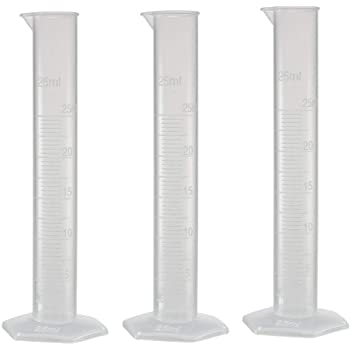
\includegraphics[width=5cm, height=5cm]{cylinders.jpg}
%%     \caption{Three graduated lab cylinders, corresponding to three
%%      eigenvectors. Prior precision eigenvalues not shown.}
%%     \label{fig:cylinder}
%% \end{figure}



\subsection{Answer to Question \ref{q:why}}\label{subsec:why}
Building on Theorem \ref{thm:char}, we can now give a compelling
explanation to the measurement clusterization we observed for the
inverse problem of the heat equation (Fig.~\ref{fig:eigenvectors}).

Consider $\fwd$ and $\prcov$ from \emph{the inverse problem of the
heat equation}. As before, we denote the eigenvalues of
$\fwd\prcov\fwd^*$ by $\lambda_j$. We input these eigenvalues into our
\emph{generic} model, and find a D-optimal design $\opt$ for our
generic model using Theorem \ref{thm:char}. In our generic model, the
measurements we take are best utilized in reducing uncertainty for the
first $k$ eigenvectors. So, a D-optimal design arising from our
\emph{generic model} completely avoids measuring eigenvectors $k+1$
and above.

Of course, in a real life problem --- such as the inverse problem of
the 1D heat equation --- it is likely impossible to find measurement
locations for which all eigenvectors $k+1$ and above are
zero. However, if the eigenvalues of $\fwd\prcov\fwd^*$ decay quickly
(recall the square-exponential decay for eigenvalues of the 1D heat
equation in eq.\eqref{eq:decay}), a D-optimal design will try to
balance measuring a small number (i.e.~$k$) of the leading
eigenvectors.

The abovementioned trade-off is explored in
Fig.~\ref{fig:eigenvectors}. We allow $m=4$ measurements in $\Omega =
[0,1]$ and observe that D-optimal measurement locations are clustered
at $x_1 = 0.31$ and $x_2 = 0.69$. Upon close inspection of the scaled
eigenvectors of $\fwd \prcov \fwd^*$, we first observe that
eigenvectors $3$ and above have negligible prior amplitude. Since we
only have $m=4$ measurements at our disposal, we interpret these
results, following Theorem \ref{thm:char}, as implying we should only
care about measuring the first and second eigenvectors. Then, we note
the D-optimal $x_1,x_2$ present a compromise between the amplitude of
the first and second eigenvectors. For example, a measurement at
$x=0.5$ would have ignored the second eigenvector altogether, since
the second eigenvector is zero at $x=0.5$.

Now we can understand measurement clusterization for the inverse
problem of the heat equation. A D-optimal design attempts to measure
the first $k$ eigenvectors of $\fwd \prcov \fwd^*$. But there may be
(spatial) limitations on where these $k$ eigenvectors have large
amplitude. For the inverse problem of the heat equation there are two
spatial locations that present a good compromise between the
amplitudes of the first and second eigenvectors, namely $x_1$ and
$x_2$ --- see Fig.~\ref{fig:eigenvectors}. We have $m=4$ measurements
at our disposal but only two spatial locations that are a good
compromise between the first and second scaled eigenvectors. Thus,
clusterization arises as a consequence of the pigeonhole principle.

\begin{figure}\label{fig:eigenvectors}
    \centering
    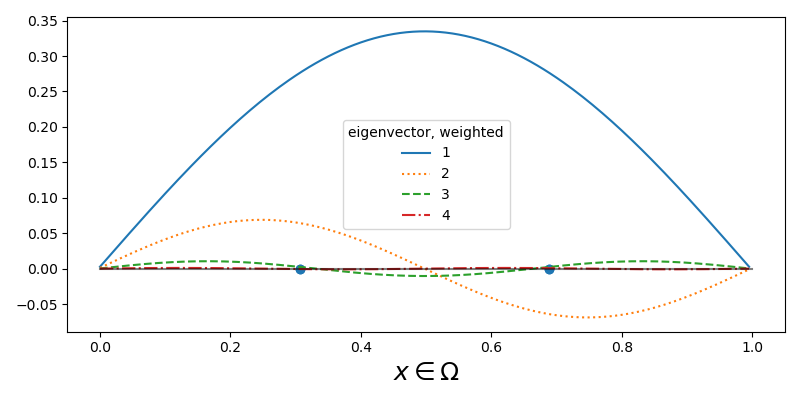
\includegraphics[width=\textwidth]{figs/eigenvectors_dst_scaled.png}
    \caption{D-optimal measurement locations ($m=4$ measurements) and
      weighted eigenvectors for finding the initial condition of the
      1D heat equation. Measurement locations and weighted
      eigenvectors are plotted over the computational domain $\Omega =
      [0, 1]$ (x-axis). Measurement clusterization occurs
      approximately at $0.31$ and $0.69$. These two locations are a
      compromise between the magnitudes of the first and second
      eigenvectors, which are the eigenvectors that a D-optimal design
      aims to measure. Allocating $m=4$ measurements into two
      locations results in clusterization, according to the pigeonhole
      principle.}
  \label{fig:why}
\end{figure}

\appendix
\section{The inverse problem of the 1D heat equation}\label{section:example}
The mathematical foundations of inversion in function spaces can be
found in \cite{Stuart10}. Our goal is to infer the intial condition of
the one-dimensional heat equation with a homogeneous Dirichlet
boundary condition:
\begin{subequations}\label{eq:heat equation}
  \begin{alignat}{2}
    u_t &= \Delta u &&\qquad \text{in } [0,1] \times [0,\infty),\\
      u &= 0 &&\qquad \text{on } \{0, 1\} \times [0,\infty),\\
        u &= u_0 &&\qquad \text{on }[0,1] \times \{0\}.
  \end{alignat}
\end{subequations}

Model the prior for the initial condition as $u_0 \sim
\normal(0,\prcov)$, for $\prcov = (-\Delta)^{-1}$ with a homogeneous
Dirichlet boundary condition. Let the final time $T = 0.03$ and denote
$\fwd$ the forward operator, so that $u(\cdot, T) = \fwd u_0$. Let
$\obs$ a measurement operator, so that $u(\x_j,T) = (\obs u)_j,
j=1,\dots,m$, where $m$ is the number of allowed measurements. Assume
iid centered Gaussian observation error, so observations are given by
$u(\x_j,T) + \eps(\x_j)$ with $\eps(\x_j) \sim \normal(0, \sigma^2)$
iid, $\sigma = 0.05$. Measurement locations $\x_j,j=1,\dots,m$ are
chosen according to the D-optimality criterion of Theorem \ref{thm:d
optimality}.

Implementation of this inverse problem can be found in the
repository \url{https://github.com/yairdaon/OED}, as well as an
optimization routine for finding D-optimal designs. Unfortinately, I
was not able to install PyOED \cite{attia2023pyoed}, nor was I able to
utilize HIPPYlib \cite{VillaPetraGhattas16, VillaPetraGhattas18,
VillaPetraGhattas21}, hence the inverse problem is implemented from
scratch.

\section{Generalizations of known lemmas}

The following lemma is generalized from \cite[Chapter 9, Theorem 4,
p. 127]{Lax07}
\lax*
\begin{proof}
  Consider a differentiable operator-valued function $X(t)$ such that
  $X(0) = 0$ and $X(t)$ is positive, self-adjoint and trace-class for
  every $t\in \R$. We denote the eigenvalues of this operator by
  $\lambda_k(X(t))$ and sometimes drop the dependence on $X(t)$, so
  $\lambda_k = \lambda_k(X(t))$.  Then $\det (I+X(t))
  = \prod_{k=1}^{\infty} (1+\lambda_k) < \infty$ and this is finite by
  the arguments given in \cite{AlexanderianGloorGhattas14}. The full
  derivative is \begin{align*} \frac{\der \det (I+X(t))}{\der t}
    % 
    % 
    % 
    &= \sum_{k=1}^{\infty} 
    \frac{\partial \det (I+X(s))}{\partial (1+\lambda_k)}\Big |_{s=t}
    \frac{\der (1+\lambda_k)}{\der t} \\
    % 
    %
    %
    &= \sum_{k=1}^{\infty} \frac{\partial \prod_{l=1}^{\infty}
      (1+\lambda_l(s))}{\partial (1+\lambda_k)}\Big |_{s=t}
    \frac{\der (1+\lambda_k)}{\der t} \\
    %
    %
    %
    &= \sum_{k=1}^{\infty} \prod_{l=1, l\neq k}^{\infty}
      (1+\lambda_l(s)) \frac{\partial (1+\lambda_k(s))}{\partial (1+\lambda_k)}\Big |_{s=t}
    \frac{\der (1+\lambda_k)}{\der t} \\
    %
    %
    %    
    &= \sum_{k=1}^{\infty} \frac{\prod_{l=1}^{\infty}
      (1+\lambda_l(s))}{(1+\lambda_k)}\Big |_{s=t}
    \dot{\lambda_k}(X(t)) \\
    % 
    % 
    % 
    &= \sum_{k=1}^{\infty} \frac{\det (I+X(t))}{1 +\lambda_k} \dot{\lambda_k}(X(t)).
  \end{align*}
  The assumption $X(0) = 0$ means $\lambda_k(X(0)) = 0,\ \forall k \geq 1$. Thus:
  \begin{align*}
    \frac{\der (I+\det X(t))}{\der t}\Big |_{t=0} 
    = \sum_{k=1}^{\infty} \dot{\lambda_k}(X(0)) 
    = \frac{\der }{\der t}\tr{X(0)}
    = \tr{\dot{X}(0)},
  \end{align*}
  where the second equality follows by monotone convergence. 
  Let $Y(t)$ a trace-class self-adjoint operator such that 
  $I+Y(t)$ is invertible.
  Define $X(t)$ via $I+X(t) = (I+Y(0))^{-1/2} (I+Y(t)) (I+Y(0))^{-1/2}$. 
  We show $X(t)$ satisfies the conditions above. It is trace-class:
  \begin{align*}
    \tr{X(t)} = \tr{(I+Y(0))^{-1} (I+Y(t)) - I}
    \leq \tr{I+Y(t) - I}< \infty,
  \end{align*}
  since $Y(t)$ is trace-class. It is also clear that
  $X(0) = 0$ and $X(t)$ is self-adjoint.
  $I+Y(t) = (I+Y(0))^{1/2}(I+X(t))(I+Y(0))^{1/2}$, so
  \begin{align*}
    \frac{\der \det (I+Y(t))}{\der t}|_{t=0} 
    &= \det (I+Y(0))\frac{\der \det (I+X(t))}{\der t}\Big |_{t=0} \\
    % 
    % 
    % 
    &= \det (I+Y(0)) \tr{\dot{X}(0)} \\
    % 
    % 
    % 
    &= \det (I+Y(0)) \tr{(I+Y(0))^{-1} \dot{Y}(0)}.
  \end{align*}
  Consequently, by the one-variable chain rule:
  \begin{align*}
    \frac{\der \log \det (I+Y(t))}{\der t}\Big |_{t=0} &=
    % 
    % 
    % 
    \frac{1}{\det (I+Y(0))}\frac{\der \det (I+Y(t))}{\der t}\Big |_{t=0} \\ 
    % 
    % 
    % 
    &= \tr{ (I+Y(t))^{-1} \dot{Y}(t)} \big |_{t=0}.
  \end{align*}
  There is nothing special about $t_0 = 0$ --- we could have chosen
  any other $t_0$ instead. Thus, the relation holds for all $t$.
\end{proof}


\begin{lemma}[Matrix Determinant Lemma in Hilbert Spaces]\label{lemma:MDL}
  Let $\hil$ a separable Hilbert space, $u,v\in \hil$ and $A: \hil \to
  \hil$ an invertible linear operator such that $\tr{A-I} <
  \infty$. Then $\det A$ and $\det A + uv^*$ are well defined and
  \begin{equation*}
    \det (A + uv^*) = (1 + \langle A^{-1} u, v \rangle ) \det A,
  \end{equation*}
  where $(A + uv^*)w := Aw + \langle v,w \rangle u$.
\end{lemma}
\begin{proof}
  In this proof we rely on definitions and results from
  \cite{simon1977}. First, consider $B := I + xy^*$ for some $x,y \in
  \hil$. We construct an eigenbasis for $B$ and use that to show $\det
  B = 1 + \langle x, y \rangle$. First let $x_1 := x$.  Now, if $x
  \parallel y$, take $\{x_n \}_{n=2}^{\infty}$ an orthogonal basis for
  $span\{x_1\} ^{\perp}$. If, on the other hand, $x \not \parallel y$, let
  \begin{equation*}
    x_2 := x - \frac{ \langle x, y\rangle}{\|y\|^2}y
  \end{equation*}
  and it is easy to verify that $x_2 \perp y$ and $span \{x,y\} = span
  \{x_1,x_2\}$. Take $\{x_n \}_{n=3}^{\infty}$ an orthogonal basis for
  $span\{x_1,x_2\} ^{\perp}$. In both cases,
  \begin{equation*}
    B x_n =
    \begin{cases}
      (1 + \langle x, y \rangle) x_n & n = 1 \\
      x_n                            & n \neq 1,
    \end{cases}
  \end{equation*}
  and so $\det B = 1 + \langle x, y \rangle$.
  
  It is easy to verify that $uv^*$ is trace-class and since $\tr{A-I}
  < \infty$, also $\tr{A + uv^* - I} < \infty$ (sum of two trace-class
  operators is trace-class). Thus $\det A$ and $\det (A+uv^*)$ are
  well defined. Let $x:=A^{-1}u$ and $y := v$:
  \begin{equation*}
    \det (A + uv^*) = \det A \ \det(I+A^{-1}uv^*) =
    (1 + \langle A^{-1}u, v \rangle) \det A .
  \end{equation*}
\end{proof}


%% \free
%% \begin{proof}
%%   Let us diagonalize $M$, so that $M = U D U^t$ with $D =
%%   \diag(d_1,\dots,d_k)$ and $U \in \R^{k \times k }$ orthogonal. Let
%%   $S \in \R^{k \times m}$ with $S_{ii} = \sqrt{d_{i}}$ and zeros
%%   otherwise. Define $A:= U S V^t$, where $V \in \R^{m \times m}$ is
%%   orthogonal and will be further restricted later. Then $AA^t = U
%%   SV^tVS^t U^t = UDU^t$, so $AA^t$ has the required eigenvalues and
%%   eigenvectors by construction. If we can choose $V$ such that $A$
%%   also satisfies the unit norm constraints we are done. These
%%   constraints are, for $j=1,\dots,m$:
%%   \begin{equation}\label{eq:V constraints}
%%    1 = [A^tA]_{jj} = [V S^tS V^t]_{jj},
%%   \end{equation}
%%   and we can expect to do this since we assumed $\ttr D = m$.

%%   Define $C = S^tS - I \in \R^{m \times m}$. Note that $\ttr C = 0$ and
%%   $C$ is diagonal with non-zero entries $d_i-1,i=1,\dots,k$. It suffices
%%   to find $V$ orthogonal such that $V C V^t$ has zero diagonal. We
%%   construct such $V$ by sequentially inserting zeros in the diagonal
%%   and not destroying zeros we already introduced, starting from the
%%   last diagonal entry and moving to the first. Since $c_{mm} \neq 0$ ,
%%   let $p < m$ such that $c_{pp}c_{mm} < 0$ (such $p$ exists because
%%   the trace is zero) and let $\theta \in (0,\pi)$. Define a Givens
%%   rotation $R^{(m)} \in \R^{m \times m}$ by
%%   \begin{equation*}
%%     r^{(m)}_{ab} :=
%%     \begin{cases}
%%       1 & a = b \neq p \text{ or } a = b \neq m \\
%%       \cos \theta & a = b = p  \\
%%      -\sin \theta & a = p, b = m\\
%%       \cos \theta & a = b = m \\
%%       \sin \theta & a = m, b = p \\ 
%%       0 & o.w
%%     \end{cases}
%%   \end{equation*}
%%   Note that conjugating a matrix by $R^{(m)}$ changes only its $m$ and
%%   $p$ rows and columns. We want to choose $\theta$ such that
%%   \begin{equation}\label{eq:mm}
%%     0 = [R^{(m)} C (R^{(m)})^t]_{mm} = \cos^2 \theta c_{mm} + 2\cos \theta \sin
%%     \theta c_{mp} + \sin^2\theta c_{pp},
%%   \end{equation}
%%   and it suffices to choose $\theta$ such that
%%   \begin{equation*}
%%     c_{mm} \cot^2 \theta + 2 c_{mp} \cot \theta + c_{pp} = 0.
%%   \end{equation*}
%%   This quadratic in $\cot\theta$ has a real solution, since
%%   $c_{pp}c_{mm} < 0$ by assumption and we can find $\theta \in
%%   (0,\pi)$ such that \eqref{eq:mm} is satisfied. We continue to find
%%   $R^{(m-1)}$ that leaves row and column $m$ unchanged and
%%   continue introducing zeros to the diagonal. The assumption $\ttr D =
%%   m \Rightarrow \ttr C = 0$ guarantees we can do that. Taking $V:=
%%   R^{(1)} R^{(2)} \dots R^{(m-1)}R^{(m)}$ completes the proof.
%% \end{proof}



%%%%%%%%%%%%%%%%%%%%%%%%%%%%%%%%%%%%%%%%%%%%%%%%%%%%%%%%%%%%%%%%%%%%%%%%%
%% \woodbury
%% \begin{proof}
%%   The proof amounts to using Woodbury's matrix identity twice and a
%%   regularization trick. The standard proof for Woodbury's matrix
%%   identity works in infinite dimensions, as long as all terms are well
%%   defined. Unfortunately, $\obs^*\obs$ is not invertible, so we force
%%   it to be. Recall Woodbury's matrix identity:
%%   $$
%%   (A + UCV)^{-1} = A^{-1} - A^{-1}U(C^{-1} + VA^{-1}U)^{-1}VA^{-1}.
%%   $$

%%   Denote $A := \prcov^{-1}$, $U := \fwd^*$, $V := \fwd$, $C :=
%%   \sigma^{-2} (\obs^*\obs+\eps I)$ for some $\eps > 0$. Then:
%%   %% \begin{align*}
%%   %%   \begin{split}
%%   \begin{equation}\label{eq:first}
%%   \fwd( \prcov^{-1} + \sigma^{-2}  \fwd^* (\obs^* \obs +\eps I) \fwd )^{-1}\fwd^* = \fwd ( \prcov - \prcov \fwd^* ( \sigma^2(\obs^*\obs + \eps I)^{-1} + \fwd \prcov \fwd^* )^{-1} \fwd \prcov ) \fwd^* \\
%%       %
%%       %
%%       %% &= X - X(\sigma^2Y_{\eps}^{-1} + X)^{-1}X
%%   %%   \end{split}
%%   %% \end{align*}
%%   \end{equation}
%%    Now denote $X := \fwd\prcov \fwd^*$ and $Y_{\eps} := \obs^*\obs +
%%    \eps I$, and $Y_{\eps}$ is invertible. Then \eqref{eq:first}
%%    becomes:
%%    \begin{equation}\label{eq:second}
%%      \fwd( \prcov^{-1} + \sigma^{-2}  \fwd^* (\obs^* \obs +\eps I) \fwd )^{-1}\fwd^* = X - X(\sigma^2Y_{\eps}^{-1} + X)^{-1}X
%%    \end{equation}

%%    Note that $X + \sigma^2 Y_{\eps}^{-1}$ is invertible, as the sum of
%%    two positive definite operators. Now, taking $A := X^{-1}, C :=
%%    \sigma^2Y_{\eps}^{-1}, U := I$ and $V := I$ and using Wodbury's
%%    matrix identity in reverse order:
%%   \begin{align*}
%%     \begin{split}
%%       \fwd( \prcov^{-1} + \sigma^{-2}  \fwd^* (\obs^* \obs +\eps I) \fwd )^{-1}\fwd^* &= X - X(\sigma^2Y_{\eps}^{-1} + X)^{-1}X \\
%%       %
%%       %
%%       %
%%       &= (X^{-1} + \sigma^{-2}Y_{\eps})^{-1} \\
%%       %
%%       %
%%       %
%%       &= (\fwd \prcov \fwd^* + \sigma^{-2} (\obs^*\obs + \eps I))^{-1}.
%%     \end{split}
%%   \end{align*}

%%   We conclude that $\forall \eps > 0$
%%   \begin{align*}
%%     \begin{split}
%%       \fwd( \prcov^{-1} + \sigma^{-2}  \fwd^* (\obs^* \obs +\eps I) \fwd )^{-1}\fwd^* 
%%      &= (\fwd \prcov \fwd^* + \sigma^{-2} (\obs^*\obs + \eps I))^{-1}.
%%     \end{split}
%%   \end{align*}
%%   Letting $\eps \to 0$ completes the proof.
%% \end{proof}


%%%%%%%%%%%%%%%%%%%%%%%%%%%%%%%%%%%%%%%%%%%%%%%%%%%%%%%%%%%%%%%%%%%%%%%%%
%% \begin{lemma}[Increase due to an observation]\label{lemma:design increase}
%%   Let $\obs = (\meas_1,\dots,\meas_m)^t$ and $\obsm :=
%%   (\meas_1,\dots,\meas_{m-1})^t$. Then
%%   \begin{align*}
%%     \tar( \obs ) - \tar (\obsm ) &=
%%     \frac12 \log \left ( 1 + \frac{
%%       \langle \fwd \postcovm \fwd^* (\obsm^* \Sigmam^{-1} \modcov - I ) \meas_m,
%%       (\obsm^* \Sigmam^{-1} \modcov - I ) \meas_m \rangle
%%     }{
%%       \sigma^2 + \meas_m \modcov \meas_m - \meas_m \modcov \obsm^* \Sigmam^{-1} \obsm \modcov \meas_m 
%%     }       
%%     \right ).
%%   \end{align*}
%% \end{lemma}
%% \begin{proof}
%%   We use the Schur complement:
%%   %% to write one inverse in terms of the other: and introduce
%%   %%  notations to make the derivation cleaner. Note that we think of
%%   %%  $\obsm$ and $\obsm^*$ as column and row vectors (respectively).
%%   \begin{align*}
%%     \Sigma( \obs ) &= \Sigma = 
%%     \begin{bmatrix}
%%       \Sigma (\obsm )           & \obsm \modcov \meas_m \\
%%       \meas_m \modcov \obsm^*   & \sigma^2 + \meas_m \modcov \meas_m
%%     \end{bmatrix}
%%     : =
%%     \begin{bmatrix}
%%       \Sigmam   & w \\
%%       w^t       & c
%%     \end{bmatrix}\\
%%     %
%%     %
%%     %
%%     \Sigma^{-1} &=
%%     \begin{bmatrix}
%%       \Sigmam^{-1} + \Sigmam^{-1} w ( c - w^t \Sigmam^{-1} w)^{-1} w^t \Sigmam^{-1} & - \Sigmam^{-1} w ( c - w^t \Sigmam^{-1} w)^{-1} \\
%%       -( c - w^t \Sigmam^{-1} w)^{-1} w^t \Sigmam^{-1}                            &  ( c - w^t \Sigmam^{-1} w)^{-1}
%%     \end{bmatrix} \\
%%     &=
%%     \begin{bmatrix}
%%       \Sigmam^{-1} & 0 \\
%%       0           & 0 
%%     \end{bmatrix}
%%     + (c -w^t \Sigmam^{-1} w )^{-1}
%%     \begin{bmatrix}
%%       \Sigmam^{-1} w \\
%%       -1
%%     \end{bmatrix}
%%     \begin{bmatrix}
%%       w^t \Sigmam^{-1} & -1 
%%     \end{bmatrix}
%%   \end{align*}
%%   %
%%   Further, define
%%   %
%%   \begin{align*}
%%     \M (\obs ):&= \prcov^{\frac12}\fwd^* \obs^* \Sigma^{-1} \obs \fwd
%%     \prcov^{\frac12}    
%%   \end{align*}
%%   %
%%   and note that:%% , using our understanding of what is a column vector and
%%   %% what is a row vector:
%%   %
%%   \begin{align*}
%%     \M(\obs) &= \prcov^{1/2} \fwd^* \obs^* \Sigma^{-1} \obs \fwd \prcov^{1/2} \\
%%     %
%%     %
%%     %
%%     &= \prcov^{1/2} \fwd^* \obs^* \left \{
%%     \begin{bmatrix}
%%       \Sigmam^{-1} & 0 \\
%%       0           & 0 
%%     \end{bmatrix}
%%     + (c -w^t \Sigmam^{-1} w )^{-1}
%%     \begin{bmatrix}
%%       \Sigmam^{-1} w \\
%%       -1
%%     \end{bmatrix}
%%     \begin{bmatrix}
%%       w^t \Sigmam^{-1} & -1 
%%     \end{bmatrix} 
%%     \right \} \obs \fwd \prcov^{1/2} \\
%%     %
%%     %
%%     %
%%     &= \M (\obsm) + (c -w^t \Sigmam^{-1} w )^{-1}
%%     \prcov^{1/2} \fwd^* \obs^*
%%     \begin{bmatrix}
%%       \Sigmam^{-1} w \\
%%       -1
%%     \end{bmatrix}
%%     \begin{bmatrix}
%%       w^t \Sigmam^{-1} & -1 
%%     \end{bmatrix} 
%%     \obs \fwd \prcov^{1/2}
%%   \end{align*}
%%   %
%%   Now, denote:
%%   %
%%   \begin{align}\label{eq:u}
%%     \begin{split}
%%       u :&= (c -w^t \Sigmam^{-1} w )^{-1/2}
%%       \prcov^{1/2} \fwd^* \obs^* 
%%       \begin{bmatrix}
%%         \Sigmam^{-1} w \\
%%         -1 
%%       \end{bmatrix} \\
%%       %
%%       %
%%       %
%%       & = (c -w^t \Sigmam^{-1} w )^{-1/2} ( \prcov^{1/2}\fwd^* \obsm^* \Sigmam^{-1} \obsm  \modcov \meas_m - \prcov^{1/2} \fwd^* \meas_m )\\
%%       %
%%       %
%%       %
%%       u^* :&=  (c -w^t \Sigmam^{-1} w )^{-1/2} (\meas_m \modcov \obsm^* \Sigmam^{-1} \obsm \fwd \prcov^{1/2} - \meas_m \fwd \prcov^{1/2} ),
%%     \end{split}
%%   \end{align}
%%   %
%%   so that
%%   %
%%   \begin{equation}\label{eq:M plus I}
%%     I + \M( \obs ) = I + \M (\obsm ) + uu^*.
%%   \end{equation}
%%   %
%%   Note that
%%   \begin{equation}\label{eq:M postcov}
%%     \prcov^{1/2} \left (I + \M( \obsm ) \right )^{-1} \prcov^{1/2} = \postcovm.
%%   \end{equation}
%%   The increase in the design criterion gained by including $\meas_m$
%%   is then: 
%%   %
%%   \begin{align*}
%%     \tar( \obs ) - \tar( \obsm )
%%     %
%%     %
%%     %
%%     &= \frac12 \log \det \Big ( I + \M ( \obs ) \Big ) / \det \Big ( I + \M (\obsm) \Big ) \\
%%     %
%%     %
%%     %
%%     &= \frac12  \log \det \left ( I + \M(\obsm) + uu^* \right ) / \det \Big ( I + \M (\obsm) \Big ) \\
%%     %
%%     %
%%     %
%%     &= \frac12 \log \left ( 1 + \left \langle \left ( I+\M(\obsm) \right )^{-1} u, u  \right \rangle \right ) \text{ (Lemma \ref{lemma:MDL})}.
%%   \end{align*}
%%   Using \eqref{eq:u} and \eqref{eq:M postcov}:
%%   \begin{align*}
%%     &\left \langle \left (I+\M (\obsm)\right )^{-1}u, u \right \rangle\\
%%     &= \frac{
%%       \langle \fwd \postcovm \fwd^* (\obsm^* \Sigmam^{-1} \obsm \modcov - I ) \meas_m,
%%       (\obsm^* \Sigmam^{-1} \obsm \modcov - I ) \meas_m \rangle
%%     }{
%%       c- w^t \Sigmam^{-1} w
%%     }\\
%%     %
%%     %
%%     %
%%     &= 
%%     \frac{
%%       \langle \fwd \postcovm \fwd^* (\obsm^* \Sigmam^{-1} \obsm \modcov - I ) \meas_m,
%%       (\obsm^* \Sigmam^{-1} \obsm \modcov - I ) \meas_m \rangle
%%     }{
%%       \sigma^2 + \meas_m \modcov \meas_m - \meas_m \modcov \obsm^* \Sigmam^{-1} \obsm \modcov \meas_m 
%%     }
%%   \end{align*}
%%   and the conclusion follows.
%% \end{proof}

%% Lemma \ref{lemma:design increase} implies the following corollary:
%% \begin{corollary}[Gain for No Model Error]\label{cor:zero mod err}
%%   If $\modcov = 0$, then
%%   \begin{equation*}
%%     \tar( \obs ) - \tar (\obsm )
%%     = -\frac12 \log (1 - \sigma^{-2} \langle \fwd \postcov \fwd^* \meas_m, \meas_m \rangle ).
%%   \end{equation*}
%% \end{corollary}
%% \begin{proof}
%%   Note that this is not immediate by substituting $\modcov = 0$ in the
%%   conclusion of Lemma \ref{lemma:design increase}, since we make a
%%   claim for $\postcov$, and not $\postcovm$. Let us first review
%%   \eqref{eq:u} and note that since $\modcov = 0$ the covariance
%%   $\Sigmam = \sigma^2I_{m-1}$ and $w = 0$, so $c - w^t\Sigmam^{-1}w =
%%   \sigma^2$:
%%   \begin{align*}
%%     u :&=-\sigma^{-1}\prcov^{1/2} \fwd^* \meas_m\\
%%     %
%%     %
%%     u^* :&= -\sigma^{-1} \meas_m \fwd \prcov^{1/2}.
%%   \end{align*}
%%   From \eqref{eq:M plus I}:
%%   \begin{equation*}
%%     I + \M(\obsm) = I +\M(\obs) - uu^*,
%%   \end{equation*}
%%   and thus:
%%   \begin{equation*}
%%     \left \langle \left ( I +\M(\obs) \right )^{-1} u, u \right \rangle
%%     = \sigma^{-2} \langle \fwd \postcov \fwd^* \meas_m, \meas_m \rangle.
%%   \end{equation*}
%%   Analogously to \eqref{eq:M postcov} we note that
%%   \begin{equation*}
%%     \prcov^{1/2} \left ( I + \M(\obs) \right )^{-1} \prcov^{1/2} = \postcov.
%%   \end{equation*}
%%   Using Lemma \ref{lemma:MDL} we conclude
%%   \begin{align*}
%%     \tar( \obs ) - \tar( \obs )
%%     &= \frac12 \log \det \left (I +\M(\obs) \right ) / \det \left (I + \M(\obsm) \right ) \\
%%     %
%%     %
%%     %
%%     &= \frac12 \log \det \left (I +\M(\obs) \right ) / \det \left (I + \M(\obs) - uu^* \right ) \\
%%     %
%%     %
%%     %
%%     &=-\frac12 \log (1 - \langle (I+\M(\obs))^{-1}u, u \rangle \\
%%     %
%%     %
%%     %
%%     &= -\frac12 \log (1 - \sigma^{-2} \langle \fwd \postcov \fwd^* \meas_m, \meas_m \rangle ).
%%   \end{align*}
%% \end{proof}

% \samemeas
%% \begin{proof} \label{cor:same meas proof}
%%   Denote $A:= \obs \modcov \obs^*$ and $v_j$ the $j$th column of $A$.
%%   Note that $v_j = \obsm \modcov \meas_m$, since $(\obsm \modcov
%%   \obsm^*)_{ij} = \meas_i(\modcov \meas_j)$, as explained in
%%   \eqref{eq:modcov explained}. One can now verify that
%%   \begin{equation}\label{eq:observation}
%%     \Sigmam^{-1} \obsm \modcov \meas_m = \Sigmam^{-1}v_j = (A +\sigma^2I_{m-1})^{-1} v_j =
%%     e_j -\sigma^2 \Sigmam^{-1}e_j.
%%   \end{equation}
%%   %
%%   Using \eqref{eq:observation}:
%%   \begin{align}\label{eq:denominator}
%%     \begin{split}
%%       \meas_m \modcov \obsm^* \Sigmam^{-1} \obsm \modcov \meas_m
%%       &= \meas_m \modcov \obsm^* ( e^j - \sigma^2 \Sigmam^{-1} e_j )\\
%%       %
%%       %
%%       %
%%       &= \meas_m \modcov \meas_j - \sigma^2 \meas_m \modcov \obsm^* \Sigmam^{-1}e_j \\
%%       %
%%       %
%%       %
%%       &= \meas_m \modcov \meas_j -\sigma^2 (e_j - \sigma^2 \Sigmam^{-1}e_j)^t e_j \\
%%       %
%%       %
%%       %
%%       &= \meas_m \modcov \meas_m -\sigma^2 + \sigma^4 e_j^t\Sigmam^{-1}e_j.
%%     \end{split}
%%   \end{align}
%%   We use \eqref{eq:observation} to simplify the terms in the enumerator of
%%   the conclusion of Lemma \ref{lemma:design increase}:
%%   \begin{align}\label{eq:enumerator}
%%     \begin{split}
%%       (\obsm^* \Sigmam^{-1} \obsm \modcov - I ) \meas_m
%%       &= \obsm^* \Sigmam^{-1} \obsm \modcov \meas_m - \meas_m \\
%%       %
%%       %
%%       %
%%       &= \obsm^* (e_j - \sigma^2 \Sigmam^{-1} e_j) -\meas_j \\ 
%%       %
%%       %
%%       %
%%       &= -\sigma^2 \obsm^* \Sigma^{-1}e_j. 
%%     \end{split}
%%   \end{align}
%%   %
%%   Substitute \eqref{eq:enumerator} and \eqref{eq:denominator} to
%%   the enumerator and denominator (respectively) of the conclusion of
%%   Lemma \ref{lemma:design increase}:
%%   %
%%   \begin{align*}
%%     \tar( \obs ) - \tar (\obsm ) &=
%%     \log \left ( 1 + \frac{
%%       \langle \fwd \postcovm \fwd^* (\obsm^* \Sigmam^{-1} \modcov - I ) \meas_m,
%%       (\obsm^* \Sigmam^{-1} \modcov - I ) \meas_m \rangle
%%     }{
%%       \sigma^2 + \meas_m \modcov \meas_m - \meas_m \modcov \obsm^* \Sigmam^{-1} \obsm \modcov \meas_m 
%%     }       
%%     \right ) \\
%%     %
%%     %
%%     %
%%     &= \log \left ( 1 + \frac{\sigma^4
%%       \langle \fwd \postcovm \fwd^* \obsm^* \Sigmam^{-1} e_j,
%%       \obsm^* \Sigmam^{-1}e_j \rangle
%%     }{
%%       2\sigma^2 - \sigma^4 e_j^t\Sigmam^{-1}e_j 
%%     }       
%%     \right ) \\
%%     %
%%     %
%%     %
%%     &= \log \left ( 1 + \frac{\sigma^2
%%       \langle \fwd \postcovm \fwd^* \obsm^* \Sigmam^{-1} e_j,
%%       \obsm^* \Sigmam^{-1}e_j \rangle
%%     }{
%%       2 - \sigma^2 e_j^t\Sigmam^{-1}e_j 
%%     }       
%%     \right ).
%%   \end{align*}
%% \end{proof}




\bibliographystyle{amsplain}
\bibliography{refs,georg_refs}

\end{document}





